\documentclass[a4paper,leqno,twocolumn]{article}
% ==== Inputs and Usepackages ====

\usepackage{tablefootnote}
\usepackage{enumerate}
\usepackage{float}
\usepackage{url}
\usepackage{hyperref}
\usepackage{dsfont}
\usepackage{mathrsfs}
\usepackage{amsmath}
\usepackage{amssymb}
\usepackage{amsthm}
\usepackage{amsfonts}
\usepackage{mathtools}
%\usepackage{mathabx}
\usepackage{MnSymbol}
\usepackage{xfrac}
\usepackage{nicefrac}
\usepackage{geometry}
\usepackage{graphicx}
\usepackage{graphics}
\usepackage{latexsym}
\usepackage{setspace}
\usepackage{tikz-cd}
\usepackage{tikz}
 \usetikzlibrary{matrix}
 \usetikzlibrary{calc}
 \usetikzlibrary{circuits.ee.IEC}
\usepackage{circuitikz}

\usepackage{a4wide}
\usepackage{fancybox}
\usepackage{fancyhdr}
\usepackage[utf8]{inputenc}




% ==== Page Settings ====

\hoffset = -1.2 in
\voffset = -0.3 in
\textwidth = 590pt
\textheight = 770pt
\setlength{\headheight}{20pt}
\setlength{\headwidth}{590pt}
\marginparwidth = 0 pt
\topmargin = -0.75 in
\setlength{\parindent}{0cm}


% ==== Presettings for files ====

\pagestyle{fancy}


\cfoot{\thepage}
\lfoot{\href{mailto:szekerb@student.ethz.ch}{szekerb@student.ethz.ch}}
\rfoot{Balázs Szekér, \today}
\lhead{Physics \uproman{3} Summary}

% ==== General Commands ====

\newcommand{\sframebox}[1]{
        \framebox[500pt][l]{\parbox{490pt}{
            #1
        }
    }

}

\newcommand{\cframebox}[2]{
        \fbox{\parbox{#1pt}{
            #2
        }
    }
}









% ====== Maths ======


% ==== Formats ====
\newcommand{\boldline}[1]{\textbf{\underline{#1}}}
\newcommand{\uproman}[1]{\uppercase\expandafter{\romannumeral#1}}
\newcommand{\lowroman}[1]{\romannumeral#1\relax}
\newcommand{\fat}[1]{\textbf{#1}}
\newcommand{\Loesung}{\begin{center}\textbf{Lösung}\end{center}}

\newcommand{\Korollar}[1]{\textbf{Korollar} \vspace{1\baselineskip} #1}
\newcommand{\Beispiel}[1]{\textbf{Beispiel} \vspace{1\baselineskip} #1}
\newcommand{\Beweis}[1]{\textbf{Beweis} \vspace{1\baselineskip} #1}
\newcommand{\Proposition}[1]{\textbf{Proposition} \vspace{1\baselineskip} #1}
\newcommand{\Satz}[1]{\textbf{Satz} \vspace{1\baselineskip} #1}
\newcommand{\Definition}[1]{\textbf{Definition} \vspace{1\baselineskip} #1}
\newcommand{\Lemma}[1]{\textbf{Lemma}\vspace{1\baselineskip} #1}
\newcommand{\Bemerkung}[1]{\textbf{Bemerkung} \vspace{1\baselineskip} #1}
\newcommand{\Theorem}[1]{\textbf{Theorem} \vspace{1\baselineskip} #1}




% ==== mathsymbols ====
\newcommand{\Q}{\mathbb{Q}}
\newcommand{\R}{\mathbb{R}}
\newcommand{\N}{\mathbb{N}}
\newcommand{\Z}{\mathbb{Z}}
\newcommand{\C}{\mathbb{C}}
\newcommand{\K}{\mathbb{K}}
\newcommand{\eS}{\mathbb{S}}
\newcommand{\X}{$X$ }
\newcommand{\Y}{$Y$ }
\newcommand{\x}{$x$ }
\newcommand{\y}{$y$ }
\newcommand{\B}{\mathcal{B}}
\newcommand{\A}{\mathcal{A}}
\renewcommand{\S}{\mathcal{S}}
\renewcommand{\P}{\mathcal{P}}



% ==== math operators ====
\newcommand{\klammer}[1]{\left( #1 \right)} 
\newcommand{\eckigeklammer}[1]{\left[ #1 \right]}
\newcommand{\geschwungeneklammer}[1]{\left\{ #1 \right\}}
\newcommand{\floor}[1]{\left\lfloor #1 \right\rfloor}
\newcommand{\ceil}[1]{\left\lceil #1 \right\rceil}
\newcommand{\scalprod}[2]{\left\langle #1 , #2 \right\rangle}
\newcommand{\abs}[1]{\left\vert #1 \right\vert} 
\newcommand{\Norm}[1]{\left\vert\left\vert #1 \right\vert\right\vert}
\newcommand{\intab}{\int_a^b}
\newcommand{\intii}{\int_{-\infty}^\infty} 
\newcommand{\cint}[2]{\int_{#1}^{#2}}
\newcommand{\csum}[2]{\sum_{#1}^{#2}}
\newcommand{\limes}[1]{\lim\limits_{#1}}
\newcommand{\limessup}[1]{\limsup\limits_{#1}}
\newcommand{\limesinf}[1]{\liminf\limits_{#1}}
\newcommand{\limesninf}{\limes{n \rightarrow \infty}}
\newcommand{\limsupninf}{\limessup{n \rightarrow \infty}}
\newcommand{\liminfninf}{\limesinf{n \rightarrow \infty}}
\newcommand{\standardNorm}{\Norm{ \ \cdot \ }}
\newcommand{\einsNorm}{\Norm{ \ \cdot \ }_1}
\newcommand{\zweiNorm}{\Norm{ \ \cdot \ }_2}
\newcommand{\Hom}{\text{Hom}}
\newcommand{\Mat}{\text{Mat}}
\newcommand{\grad}{\text{grad}}
\newcommand{\vol}{\text{vol}}
\newcommand{\supp}{\text{supp}}
\newcommand{\rot}{\text{rot}}
\renewcommand{\div}{\text{div}}



% ==== Analysis ====
\newcommand{\supremum}{\text{sup}}
\newcommand{\infimum}{\text{inf}}
\newcommand{\maximum}{\text{max}}
\newcommand{\minimum}{\text{min}}

\newcommand{\xinX}{$x \in X$ }
\newcommand{\yinY}{$y \in Y$ }
\newcommand{\xyinX}{$x,y \in X$ }
\newcommand{\yinX}{$y \in X$ }
\newcommand{\xinR}{$x \in \R$ }
\newcommand{\xyinR}{$x,y \in \R$ }
\newcommand{\zinC}{$z \in \C$ }
\newcommand{\ninN}{$n \in \N$ }
\newcommand{\NinN}{$N \in \N$}
\newcommand{\angeordneterK}{$(K,\leq)$ }
\newcommand{\xFolge}{(x_n)_{n=0}^{\infty}}
\newcommand{\yFolge}{(y_n)_{n=0}^{\infty}}
\newcommand{\zFolge}{(z_n)_{n=0}^{\infty}}
\newcommand{\aFolge}{(a_n)_{n=0}^{\infty}}
\newcommand{\fFolge}{(f_n)_{n=0}^{\infty}}

\newcommand{\XsubR}{$X \subset \R$ }
\newcommand{\XsubeqR}{$X \subseteq \R$ }

\newcommand{\XFam}{\mathcal{X}}
\newcommand{\PFam}{\mathcal{P}}

\newcommand{\offenesintervall}[2]{$\left( #1 , #2 \right)$ }
\newcommand{\abgeschlossenesintervall}[2]{$\left( #1 , #2 \right)$ }

\newcommand{\XTopRaum}{(X,\tau)}


% ==== Lineare Algebra ====
\newcommand{\vinV}{$v \in V$ }
\newcommand{\uinU}{$u \in U$ }
\newcommand{\winW}{$w \in W$ }
\newcommand{\vwinV}{$v,w \in V$ }

\newcommand{\BasisV}{v_1 , \dots , v_n}
\newcommand{\BasisU}{u_1 , \dots , u_n}
\newcommand{\BasisW}{w_1 , \dots , w_n}

\newcommand{\transpose}[1]{#1^t}
\newcommand{\inverse}[1]{#1^{-1}}
\newcommand{\ddvec}[3]{\left( #1,#2,#3 \right)}
\newcommand{\tdvec}[2]{\left( #1 , #2 \right)}

\newcommand{\Edrei}{\begin{pmatrix}
    1 & 0 & 0 \\
    0 & 1 & 0 \\
    0 & 0 & 1
\end{pmatrix}}

\newcommand{\id}{\text{id}}
\newcommand{\GL}{\text{GL}}
\newcommand{\End}{\text{End}}
\renewcommand{\Im}{\text{Im}}
\renewcommand{\Re}{\text{Re}}
\renewcommand{\ker}{\text{Ker}}
\newcommand{\rang}{\text{rang}}
\newcommand{\ad}{\text{ad}}
\newcommand{\Eig}{\text{Eig}}
\newcommand{\Bil}{\text{Bil}}
\newcommand{\sign}{\text{sign}}
\newcommand{\tr}{\text{tr}}



% ====== Physics ======

% ==== Physicssymbols ====
\newcommand{\epsilonnull}{\epsilon_0}
\newcommand{\munull}{\mu_0}
\newcommand{\rn}{r_0}
\newcommand{\Rn}{R_0}
\newcommand{\rhonull}{\rho_0}
\newcommand{\Rhonull}{\varrho_0}


% ==== Notation ====
\newcommand{\Etot}{E_{\text{Tot}}}
\newcommand{\Wtot}{W_{\text{Tot}}}
\newcommand{\Ftot}{F_{\text{Tot}}}
\newcommand{\vtot}{v_{\text{Tot}}}
\newcommand{\atot}{a_{\text{Tot}}}
\newcommand{\mtot}{m_{\text{Tot}}}
\newcommand{\Mtot}{M_{\text{Tot}}}

\newcommand{\Ekin}{E_{\text{Kin}}}
\newcommand{\Epot}{E_{\text{Pot}}}
\newcommand{\Edef}{E_{\text{Def}}}

\newcommand{\Fg}{F_g}
\newcommand{\FN}{F_N}
\newcommand{\Fz}{F_z}
\newcommand{\FC}{F_C}

\newcommand{\xn}{x_0}
\newcommand{\xN}{x_n}
\newcommand{\vn}{v_0}
\newcommand{\vN}{v_n}
\newcommand{\an}{a_0}
\newcommand{\aN}{a_n}

\newcommand{\dt}{\Delta t}
\newcommand{\dx}{\Delta x}
\newcommand{\dv}{\Delta v}
\newcommand{\da}{\Delta a}
\newcommand{\dE}{\Delta E}
\newcommand{\dW}{\Delta W}
\newcommand{\dF}{\Delta F}


% ==== Relativity ====
\newcommand{\relsqrt}{\sqrt{1-\frac{v^2}{c^2}}}
\newcommand{\relgamma}{\frac{1}{\relsqrt}}


% ==== Constants ====
\newcommand{\g}{9.81}





\renewcommand{\epsilon}{\varepsilon}
\clubpenalty = 10000
\widowpenalty = 10000

\theoremstyle{definition}

\newtheorem*{theorem}{Theorem}
\newtheorem*{definition}{Definition}
\newtheorem*{lemma}{Lemma}
\newtheorem*{proposition}{Proposition}
\newtheorem*{beispiel}{Beispiel}
\newtheorem*{korollar}{Korollar}

\setcounter{section}{-1}

\begin{document}

\section{Basics}

\begin{align*}
    \partial_x \delta(x-y) = - \partial_y \delta(x-y)
    \hspace{10pt} , \hspace{10pt}
    \epsilon_{kij} \epsilon_{klm} = \delta_{il} \delta_{jm} - \delta_{im} \delta_{jl}
\end{align*}
\begin{align*}
    a \times (b \times c) &= (a \cdot c) b - (a \cdot b) c
    \\
    (a \times b) \cdot (c \times d) &= (a \cdot c) (b \cdot d) - (a \cdot d) (b \cdot c)
    \\
    R a \times R b = R (a \times b)
    \hspace{10pt} &, \hspace{10pt}
    \nabla \times \nabla \psi = 0
    \\
    \nabla \times (\nabla \times A) &= \nabla \klammer{\nabla \cdot A} - \Delta A
    \\
    \nabla (A \cdot B) = (A \cdot \nabla) B &+ (B \cdot \nabla) A + A \times (\nabla \times B) + B \times (\nabla \times A)
\end{align*}
with $a,b,c,d$ vectors, $A,B$ vector fields, $R \in SO(3)$ and $\psi$ a
scalar potential.

\subsection{Spherical Coordinates}
\begin{align*}
    \vec{e}_r \times \vec{e}_\theta = \vec{e}_\varphi
    \hspace{10pt} , \hspace{10pt}
    \vec{e}_\theta \times \vec{e}_\varphi = \vec{e}_r
    \hspace{10pt} , \hspace{10pt}
    \vec{e}_\varphi \times \vec{e}_r = \vec{e}_\theta
\end{align*}
For $\vec{V} = (V_r,V_\theta,V_\varphi)$:
\begin{align*}
    \vec{\nabla} \cdot \vec{V} &=
    \frac{1}{r^2} \frac{\partial (r^2 V_r)}{\partial r}
        + \frac{1}{r \sin(\theta)} \frac{\partial (\sin(\theta) V_\theta)}{\partial \theta}
        + \frac{1}{r \sin(\theta)} \frac{\partial V_\varphi}{\partial \varphi}
    \\
    \vec{\nabla} \times \vec{V} &=
    \frac{1}{r \sin(\theta)} \eckigeklammer{\frac{\partial (\sin(\theta) V_\varphi)}{\partial \theta} - \frac{\partial V_\theta}{\partial \varphi}} \vec{e}_r
    \\
        &\hspace{10pt} + \frac{1}{r} \eckigeklammer{\frac{1}{\sin(\theta)} \frac{\partial V_r}{\partial \varphi} - \frac{\partial(r V_\varphi)}{\partial r}} \vec{e}_{\theta}
        + \frac{1}{r} \eckigeklammer{\frac{\partial(r V_\theta)}{\partial r} - \frac{\partial V_r}{\partial \theta}} \vec{e}_\varphi
\end{align*}

\subsection{Cylinder Coordinates}
\begin{align*}
    \vec{e}_r \times \vec{e}_\phi = \vec{e}_z
    \hspace{10pt} , \hspace{10pt}
    \vec{e}_\phi \times \vec{e}_z = \vec{e}_r
    \hspace{10pt} , \hspace{10pt}
    \vec{e}_z \times \vec{e}_r = \vec{e}_\phi
\end{align*}
For $\vec{V} = (V_r,V_\phi,V_z)$:
\begin{align*}
    \vec{\nabla} \cdot \vec{V} &=
    \frac{1}{r} \frac{\partial(r V_r)}{\partial r} + \frac{1}{r} \frac{\partial V_\phi}{\partial \phi} + \frac{\partial V_z}{\partial z}
    \\
    \vec{\nabla} \times \vec{V} &=
    \eckigeklammer{\frac{1}{r} \frac{\partial V_z}{\partial \phi} - \frac{\partial V_\phi}{\partial z}} \vec{e}_r
    + \eckigeklammer{\frac{\partial V_r}{\partial z} - \frac{\partial V_z}{\partial r}} \vec{e}_\phi
    + \frac{1}{r} \eckigeklammer{\frac{\partial(r V_\phi)}{\partial r} - \frac{\partial V_r}{\partial \phi}} \vec{e}_z
\end{align*}







\section{Electromagnetic Force}

\paragraph{Lorentz Force}
$\vec{F} = q \klammer{\vec{E} + \vec{v} \times \vec{B}}$

\paragraph{Maxwell Equations}
\begin{align*}
    \vec{\nabla} \cdot \vec{E} = \frac{\rho}{\epsilonnull}
    \hspace{5pt} , \hspace{5pt}
    \vec{\nabla} \times \vec{E} = - \frac{\partial \vec{B}}{\partial t}
    \hspace{5pt} , \hspace{5pt}
    \vec{\nabla} \cdot \vec{B} = 0
    \hspace{5pt} , \hspace{5pt}
    \vec{\nabla} \times \vec{B} = \frac{\vec{j}}{c^2 \epsilonnull} + \frac{1}{c^2} \frac{\partial \vec{E}}{\partial t}
\end{align*}


\section{Electrostatics}

Fixed charge distribution and static electric field.
\begin{align*}
    \vec{\nabla} \cdot \vec{E} = \frac{\rho}{\epsilonnull}
    \hspace{10pt} , \hspace{10pt}
    \vec{\nabla} \times \vec{E} = 0
\end{align*}

\subsection{Coulomb's Law}

\begin{align*}
    \vec{F} = \frac{q}{4 \pi \epsilonnull} \frac{q_1}{\abs{\vec{x} - \vec{y}_1}^3} (\vec{x} - \vec{y}_1)
    \hspace{10pt} &, \hspace{10pt}
    \vec{E} = \frac{1}{4 \pi \epsilonnull} \frac{q_1}{\abs{\vec{x} - \vec{y}_1}^3} (\vec{x} - \vec{y}_1)
    \\
    \vec{E} = \frac{1}{4 \pi \epsilonnull} \sum_{i=1}^N \frac{q_i}{\abs{\vec{x} - \vec{y}_i}^3} (\vec{x} - \vec{y}_i)
    \hspace{10pt} &, \hspace{10pt}
    \vec{E} = \frac{1}{4 \pi \epsilonnull} \int \frac{\rho(\vec{y})}{\abs{\vec{x} - \vec{y}}^3} (\vec{x} - \vec{y}) \ d^3 \vec{y}
\end{align*}

\subsubsection{Dirac Delta}

\begin{align*}
    \intii f(x) \delta(x-y) \ dx = f(y)
    \hspace{5pt} , \hspace{5pt}
    \delta (\vec{x} - \vec{y}) =
    \delta^{(D)} (\vec{x} - \vec{y}) = \prod_{i=1}^D \delta(x_i - y_i)
\end{align*}

\paragraph{Charge density} of a single charge $q$ at a position $\vec{y}$:
$\rho(\vec{x}) = q \delta(\vec{x} - \vec{y})$.

\paragraph{Charge distribution} of many point-like charges $q_i$ at positions $\vec{y}_i$:
$\rho(\vec{x}) = \sum_i q_i \delta(\vec{x} - \vec{y}_i)$

\subsection{Gauss' law from Coulomb's law}
\begin{align*}
    \vec{\nabla}_{\vec{x}} \frac{1}{\abs{\vec{x} - \vec{y}}} &= - \frac{(\vec{x} - \vec{y})}{\abs{\vec{x} - \vec{y}}^3}
    \ \Rightarrow \ \vec{E} = - \vec{\nabla} \Phi(\vec{x})
    \\
    &\Rightarrow \
    \Phi(\vec{x}) = \frac{1}{4 \pi \epsilonnull} \int \frac{\rho(\vec{y})}{\abs{\vec{x} - \vec{y}}} \ d^3 \vec{y}
    \\
    &\Rightarrow \ \vec{\nabla} \cdot \vec{E} = - \vec{\nabla}^2 \Phi = - \Delta \Phi
    = \frac{\rho}{\epsilonnull}
\end{align*}
Further: $\mathbf{\nabla}^2_{\vec{x}} \frac{1}{\abs{\vec{x} - \vec{y}}}
= - 4 \pi \delta(\vec{x} - \vec{y})$

\subsubsection{Integral form of Gauss' law}

\begin{align*}
    \int_{S(V)} \vec{E} \cdot d \vec{S}
    = \int_{V(S)} \vec{\nabla} \cdot \vec{E} \ d^3 \vec{x}
    = \frac{1}{\epsilonnull} \int_{V(S)} \rho(\vec{x}) \ d^3 \vec{x}
\end{align*}

\subsection{Scalar potential}

\begin{align*}
    \vec{\nabla} \times \vec{E} &= - \vec{\nabla} \times \vec{\nabla} \Phi = 0
    \\
    \int_S \vec{\nabla} \times \vec{E} \cdot d \vec{S}
    &= \oint_{\partial S} \vec{E} \cdot d \vec{l} = 0
\end{align*}

Field exerts a force $\vec{F} = q \vec{E} = - q \vec{\nabla} \Phi$.
Work needed to transport a test charge from a position $\vec{x}_A$ to
a position $\vec{x}_B$:
\begin{align*}
    W_{A \rightarrow B} = q \int_{\vec{x}_A}^{\vec{x}_B} \vec{\nabla} \Phi \cdot d \vec{l}
    = q \klammer{\Phi(\vec{x}_B) - \Phi(\vec{x}_A)}
\end{align*}
Work done is independent of the chosen path.

\subsection{Potential energy of a charge distribution}

Potential energy of a system is the energy required to bring the charges to
their positions from infinity. Discrete case:
\begin{align*}
    W = \frac{1}{4 \pi \epsilon_0} \sum_{i=2}^{N} \sum_{j<i} \frac{q_i q_j}{\abs{\vec{x}_i - \vec{x}_j}}
    = \frac{1}{8 \pi \epsilon_0} \sum_{i \neq j} \frac{q_i q_j}{\abs{\vec{x}_i - \vec{x}_j}}
\end{align*}
Continous case:
\begin{align*}
    W &= \frac{1}{8 \pi \epsilon_0} \int \frac{\rho(\vec{x}) \rho(\vec{y})}{\abs{\vec{x} - \vec{y}}} \ d^3 \vec{x} d^2 \vec{y}
    = \frac{1}{2} \int \rho(\vec{x}) \Phi(\vec{x}) \ d^3 \vec{x}
    \\
    &= - \frac{\epsilon_0}{2} \int \Phi(\vec{x}) \vec{\nabla}^2 \Phi(\vec{x}) \ d^3 \vec{x}
    = \frac{\epsilon_0}{2} \int \abs{\vec{E}}^2 \ d^3 \vec{x}
\end{align*}

\paragraph{Energy density of the electric field}
$w = \frac{\epsilon_0}{2} \abs{\vec{E}}^2$


\subsubsection{Self-energy}
Infinities in the total energy occur if we consider discrete distributions with
a density $\rho(\vec{x}) = \sum_i q_i \delta(\vec{x} - \vec{x}_i)$

\subsection{Charged conductors}

Electrons move freely within their mass. $\vec{E}_{\text{inside}} = 0
\Rightarrow \Phi$ const. Flux of electric field through Gauss surface:
\begin{align*}
    \text{Flux} = \int \vec{E} \cdot d \vec{S} = E \Delta S
\end{align*}
Charge enclosed:
\begin{align*}
    \text{Charge} = \sigma(\vec{x}) \Delta S
\end{align*}
with $\sigma(\vec{x})$ the charge surface density. Electric field on the
surface:
\begin{align*}
    E = \frac{\sigma(\vec{x})}{\epsilon_0}
\end{align*}
Energy density on the surface of the conductor:
\begin{align*}
    w = \frac{\epsilon_0}{2} \abs{\vec{E}}^2
    = \frac{\sigma^2(\vec{x})}{2 \epsilon_0}
\end{align*}
Small deformation $\Delta x \Delta S$ leads to a difference in electrostatic
energy:
\begin{align*}
    \Delta W = \int_{V_{\text{out}}} w \ d^3 \vec{x} - \int_{V_{\text{out}} - \Delta x \Delta S} w \ d^3 \vec{x}
    = - \Delta S \Delta x \frac{\sigma^2}{2 \epsilon_0}
\end{align*}
Force needed to undo deformation: $\Delta W = F \Delta x$. Pressure on the
surface:
\begin{align*}
    \frac{\abs{F}}{\Delta S} = \frac{\abs{\Delta W}}{\Delta x \Delta S}
    = \frac{\sigma^2}{2 \epsilonnull}
\end{align*}


\section{Boundary condition problems in electrostatics}

\subsection{Dirichlet and Neumann boundary conditions}

If we know the potential on the boundary: Dirichlet B.C

If we know $\vec{E} = - \vec{\nabla} \phi$ on the boundary: Neumann B.C.

\subsection{Green's functions}

\begin{align*}
    \vec{\nabla}_{\vec{x}}^2 G(\vec{x},\vec{y}) = -4 \pi \delta(\vec{x} - \vec{y})
    \hspace{10pt} , \hspace{10pt}
    G(\vec{x},\vec{y}) = \frac{1}{\abs{\vec{x} - \vec{y}}} + F(\vec{x},\vec{y})
\end{align*}
such that $\vec{\nabla}_{\vec{x}}^2 F(\vec{x},\vec{y}) = 0$
\begin{align*}
    \Phi(\vec{y})
    = &\frac{1}{4 \pi \epsilonnull} \int_V d^3 \vec{x} \ G(\vec{x},\vec{y}) \rho(\vec{x})
        \\
        &- \frac{1}{4 \pi} \int_{S(V)} d \vec{S} \cdot
        \eckigeklammer{\Phi(\vec{x}) \vec{\nabla}_{\vec{x}} G(\vec{x},\vec{y})
        - G(\vec{x},\vec{y}) \vec{\nabla} \Phi(\vec{x})}
\end{align*}

\subsubsection{Dirichlet boundary conditions}
We search for a Green's function $G_D (\vec{x},\vec{y})$ which vanishes on
the surface $S(V)$. Then we have:
\begin{align*}
    \Phi(\vec{y}) = \frac{1}{4 \pi \epsilonnull} \int_V d^3 \vec{x} \
        G_D (\vec{x},\vec{y}) \rho(\vec{x})
        - \frac{1}{4 \pi} \int_{S(V)} d \vec{S} \cdot \Phi(\vec{x})
        \vec{\nabla}_{\vec{x}} G_D (\vec{x},\vec{y})
\end{align*}

\subsubsection{Neumann boundary conditions}
\begin{align*}
    \Phi(\vec{y}) =
    &\frac{1}{4 \pi \epsilonnull} \int_V d^3 \vec{x} \ G_N (\vec{x},\vec{y}) \rho(\vec{x})
    \\
    &+ \frac{1}{4 \pi} \int_{S(V)} d \vec{S} \cdot G_N (\vec{x},\vec{y}) \vec{\nabla}_{\vec{x}} \Phi(\vec{x})
    + \langle \Phi \rangle_{S(V)}
\end{align*}
With $\langle \Phi \rangle_{S(V)} = \frac{\int_S(V) d \vec{S} \cdot \Phi \hat{n}}{S}$
an unimportant physical constant.

\subsection{Explicit solutions}

\subsubsection{Conductor filling half of space}

Left side: free space, right side: conductor. Let $x_1$ point to the right,
$x_2$ to the top and $x_3$ out of the plane. $\forall \vec{y} = (y_1,y_2,y_3)
\in$ LHS, we define $\vec{y}^\ast = (-y_1,y_2,y_3) \in$ RHS and
\begin{align*}
    F(\vec{x},\vec{y}) = - \frac{1}{\vec{x} - \vec{y}}
    \hspace{10pt} \Rightarrow \hspace{10pt}
    G(\vec{x},\vec{y}) = \frac{1}{\abs{\vec{x} - \vec{y}}} -
        \frac{1}{\abs{\vec{x} - \vec{y}^\ast}}
\end{align*}
This $G$ fulfills $G = 0$ on the boundary ($y_1 = 0$) and $\vec{\nabla}^2 F
= 4 \pi \delta(\vec{x} - \vec{y}^\ast) = 0$ because $\vec{x}$ and $\vec{y}$
are in different half planes. Since $\abs{\vec{x} - \vec{y}^\ast} =
\abs{\vec{y} - \vec{x}^\ast}$ we obtain:
\begin{align*}
    \Phi(\vec{y}) = &\frac{1}{4 \pi \epsilonnull} \int_{\text{free-space}} d^3 \vec{x} \ \eckigeklammer{\frac{\rho(\vec{x})}{\abs{\vec{x} - \vec{y}}} + \frac{-\rho(\vec{x})}{\abs{\vec{x} - \vec{y}^\ast}} }
        \\
        &- \frac{1}{4 \pi} \int_S d \vec{S} \cdot \Phi(\vec{x}) \vec{\nabla} \eckigeklammer{\frac{1}{\abs{\vec{x} - \vec{y}}} - \frac{1}{\abs{\vec{x} - \vec{y}^\ast}}}
        \\
        = &\frac{1}{4 \pi \epsilonnull} \int_{\text{free-space}} d^3 \vec{x} \ \eckigeklammer{\frac{\rho(\vec{x})}{\abs{\vec{x} - \vec{y}}} + \frac{-\rho(\vec{x})}{\abs{\vec{x}^\ast - \vec{y}}}}
        \\
        &- \frac{1}{4 \pi} \int_S d \vec{S} \cdot \Phi(\vec{x}) \vec{\nabla} \eckigeklammer{\frac{1}{\abs{\vec{x} - \vec{y}}} - \frac{1}{\abs{\vec{x}^\ast - \vec{y}}}}
        \\
        = &V + \frac{1}{4 \pi \epsilonnull} \int_{\text{free-space}} d^3 \vec{x} \ \eckigeklammer{\frac{\rho(\vec{x})}{\abs{\vec{x} - \vec{y}}} + \frac{-\rho(\vec{x})}{\abs{\vec{x}^\ast - \vec{y}}}}
\end{align*}
where we used that the potential $\Phi(\vec{x})$ is constant on the surface
$S$ and takes a value of $V$. In case of discrete charges:
\begin{align*}
    \rho(\vec{x}) = \sum_i q_i \delta(\vec{x} - \vec{x}_i)
    \hspace{10pt} \Rightarrow \hspace{10pt}
    \Phi(\vec{y}) = \frac{1}{4 \pi \epsilonnull} \sum_i \frac{q_i}{\abs{\vec{y} - \vec{x}}} + \frac{-q_i}{\abs{\vec{y} - \vec{x}_i^\ast}}
\end{align*}

\subsubsection{Method of images}

Consider a sphere of radius $R$ around the origin. Place a charge $+q$ at
a position $\vec{d}$ and a charge of opposite charge $-\frac{R}{d} q$ at
a position $\frac{R^2}{d^2} \vec{d}$. Contribution of these two charges
to the scalar potential at a position $\vec{r}$:
\begin{align*}
    \Phi(\vec{r}) = \frac{q}{4 \pi \epsilonnull}
        \eckigeklammer{\frac{1}{\abs{\vec{r} - \vec{d}}}
        - \frac{\frac{R}{d}}{\abs{\vec{r} - \frac{R^2}{d^2} \vec{d}}}}
    \hspace{10pt} , \hspace{10pt}
    \Phi(\vec{R}) = 0
\end{align*}
On the surface of a sphere with radius $R$, the potential vanishes.
Solution for the problem with the charge $+q$ at a distance $d$ from
the centre of a conductor of radius $R$:
\begin{align*}
    \Phi(\vec{r}) = \begin{cases}
        \frac{q}{4 \pi \epsilonnull}
        \eckigeklammer{\frac{1}{\abs{\vec{r} - \vec{d}}}
        - \frac{\frac{R}{d}}{\abs{\vec{r} - \frac{R^2}{d^2} \vec{d}}}}
        \hspace{10pt} &\forall \vec{r} : r \geq R
        \\
        0 \hspace{10pt} &\forall \vec{r} : r < R
    \end{cases}
\end{align*}
General solution:
\begin{align*}
    \Phi(\vec{r}) = \frac{q}{4 \pi \epsilonnull} G_D (\vec{d},\vec{r})
    \Rightarrow
    G_D (\vec{d},\vec{r}) = \frac{4 \pi \epsilonnull}{q} \Phi(\vec{r})
    = \frac{1}{\abs{\vec{r} - \vec{d}}} - \frac{\frac{R}{d}}{\abs{\vec{r} - \frac{R^2}{d^2} \vec{d}}}
\end{align*}

\subsection{Green's functions from Laplacian eigenfunctions}

Consider eigenfunctions $\psi_n(\vec{x})$ of the Laplace operator:
\begin{align*}
    \vec{\nabla}^2 \psi_n = \lambda_n \psi_n
    \hspace{10pt} , \hspace{10pt}
    \psi_n (\vec{x}) = 0 \ \forall \vec{x} \in S(V)
\end{align*}
with the condition that they vanish on the boundary. Eigenvalues are not
degenerate and real. Orthogonality condition:
\begin{align*}
    \int_V d^3 \vec{x} \ \psi_m^\ast (\vec{x}) \psi_n (\vec{x}) = \delta_{nm}
\end{align*}
Eigenfunctions form a complete basis: Any other function $f(\vec{x})$ which
vanishes on the boundary $S(V)$ can be written as a linear superposition
of the Laplace eigenfunctions:
\begin{align*}
    f(\vec{x}) = \sum_n c_n \psi_n (\vec{x})
    \hspace{10pt} , \hspace{10pt}
    c_n = \int_V d^3 \vec{x} \ \psi_n^\ast (\vec{x}) f(\vec{x})
\end{align*}
Completeness condition:
\begin{align*}
    \sum_n \psi_n^\ast (\vec{x}) \psi_n (\vec{x}) = \delta (\vec{x} - \vec{y})
\end{align*}
Green's function:
\begin{align*}
    G_D (\vec{x},\vec{y}) = - 4 \pi \sum_n \frac{\psi_n^\ast (\vec{y}) \psi_n (\vec{x})}{\lambda_n}
\end{align*}

\subsubsection{Infinite Space}
\begin{align*}
    G_D (\vec{x},\vec{y}) = \frac{1}{\abs{\vec{x} - \vec{y}}}
    \hspace{10pt} , \hspace{10pt}
    \psi_{\vec{k}} (\vec{x}) = \frac{1}{(2 \pi)^{\frac{3}{2}}} e^{i \vec{k} \cdot \vec{x}}
    \hspace{10pt} , \hspace{10pt}
    \lambda_{\vec{k}} = - \abs{\vec{k}}^2
\end{align*}
\begin{align*}
    \intii dx \ e^{ixa} = 2 \pi \delta(a)
\end{align*}

\subsubsection{Orthogonal Parallelepide}
Consider an orthogonal parallelepide with sidelengths $a \times b \times c$.
\begin{align*}
    \psi_{lmn} = \sqrt{\frac{8}{abc}} \sin \klammer{\frac{l \pi x}{a}}
        \sin \klammer{\frac{m \pi x}{b}} \sin \klammer{\frac{n \pi x}{c}}
\end{align*}
\begin{align*}
    \lambda_{lmn} = - \pi^2 \klammer{\frac{l^2}{a^2} + \frac{m^2}{b^2} + \frac{n^2}{c^2}}
\end{align*}
\begin{align*}
    G (\vec{x},\vec{y}) = - 4 \pi \sum_{l,m,n=1}^\infty \frac{\psi_{lmn}(\vec{x}) \psi_{lmn}(\vec{y})}{\lambda_{lmn}}
\end{align*}

\subsection{Laplace operator and spherical symmetry}

Spherical Laplace operator:
\begin{align*}
    \vec{\nabla}^2 = \frac{1}{r} \frac{\partial^2}{\partial r^2} r + \frac{\hat{A}}{r^2}
    \hspace{10pt} , \hspace{10pt}
    \hat{A} = \frac{1}{\sin(\theta)} \frac{\partial}{\partial \theta} \sin(\theta) \frac{\partial}{\partial \theta} + \frac{1}{\sin^2 (\theta)} \frac{\partial^2}{\partial^2 \phi}
\end{align*}
Setting $x = \cos(\theta)$ we obtain:
\begin{align*}
    \hat{A} = \frac{\partial}{\partial x} (1-x^2) \frac{\partial}{\partial x} + \frac{1}{1-x^2} \frac{\partial^2}{\partial^2 \phi}
\end{align*}
Separation of variables: $\psi(r,\theta,\phi) = \frac{R(r)}{r} Y(\theta,\phi)$
\begin{align*}
    r \eckigeklammer{\frac{1}{R} \frac{\partial^2 R}{\partial r^2} - \lambda} = - \frac{1}{Y} \hat{A} Y
    = l(l+1)
\end{align*}
\begin{align*}
    \frac{1}{R} \frac{\partial^2 R}{\partial r^2} - \frac{l(l+1)}{r} - \lambda = 0
    \hspace{10pt} , \hspace{10pt}
    \hat{A} Y = - l(l+1) Y
\end{align*}

\subsubsection{Radial Differential Equation}
Ansatz $R = r^a$ yiels $a = -l,l+1$, thus:
\begin{align*}
    \psi(r,\theta,\phi) = \sum_l \frac{1}{r} \klammer{A_l r^{-l} + B_l r^{l+1}} Y_l (\theta,\phi)
\end{align*}
In the case $r \rightarrow 0$ we approximate
\begin{align*}
    r^{a-2} a(a-1) - l(l+1) r^{a-2} = \lambda r^a \approx 0
\end{align*}
because $r^a$ is of higher order than $r^{a-2}$.

\subsubsection{Angular Differential Equation}
Again separation of variables: $Y(\theta,\phi) = \Theta(\theta) \Phi(\phi)$
\begin{align*}
    \frac{1+x^2}{\Theta} \eckigeklammer{\frac{\partial}{\partial x} (1-x^2) \frac{\partial}{\partial x} + l(l+1)} \Theta
    = - \frac{1}{\Phi} \frac{\partial^2 \Phi}{\partial \phi^2}
    = - m^2
\end{align*}
\begin{align*}
    \frac{\partial^2 \Phi}{\partial \phi^2} = - m^2 \Phi
    \hspace{10pt} \Rightarrow \hspace{10pt}
    \Phi(\phi) = e^{i m \phi}
    \ \ , \ m \in \Z
\end{align*}

\paragraph{Interlude Legendre Polynomials}
\begin{align*}
    P_l (x) = \frac{1}{2^l l!} \frac{d^l}{d x^l} (x^2 - 1)^l
    = \frac{1}{2^l} \sum_{k=0}^l \binom{l}{k}^2 (x-1)^{l-k} (x+1)^k
\end{align*}
Normalization condition: $P_l (1) = 1$. Legendre polynomials vanish when
integrated with any other polynomial of a lesser degree in the range $[-1,1]$:
\begin{align*}
    \int_{-1}^1 dx \ x^k P_l (x) = 0 \ \forall k = 0,1,\dots,(l-1)
\end{align*}
Orthogonality:
\begin{align*}
    \int_{-1}^1 dx \ P_l (x) P_m (x) = \frac{2}{2l+1} \delta_{lm}
\end{align*}
Legendre Polynomials form a basis for all continuous functions $f(x)$ in
$[-1,1]$:
\begin{align*}
    f(x) = \sum_{n=0}^\infty c_n P_n (x)
    \hspace{10pt} , \hspace{10pt}
    c_n = \frac{2n+1}{2} \int_{-1}^1 dx \ P_n (x) f(x)
\end{align*}
Completeness condition:
\begin{align*}
    \sum_{n=0}^\infty P_n (x) P_n (y) \frac{2n+1}{2} = \delta (x-y)
\end{align*}

\paragraph{Associated Legendre Polynomials}
\begin{align*}
    P_l^m (x) &= (-1)^m (1-x^2)^{\frac{m}{2}} \frac{\partial^m}{\partial x^m} P_l (x)
    \\
    &= \frac{(-1)^m}{2^l l!} (1-x^2)^{\frac{m}{2}} \frac{\partial^{l+m}}{\partial x^{l+m}} (x^2 - 1)^l
\end{align*}
for $m = -l,-l+1,\dots,0,\dots,l-1,l$.
\begin{align*}
    P_l^{-m} = (-1)^m \frac{(l-m)!}{(l+m)!} P_l^m (x)
\end{align*}
Orthogonality condition:
\begin{align*}
    \int_{-1}^1 dx \ P_k^m (x) P_l^m (x) &= \frac{2(m+l)!}{(2l+1)(l-m)!} \delta_{kl}
    \\
    \int_{-1}^1 dx \ \frac{P_l^m (x) P_l^n}{1-x^2} &= \frac{(l+m)!}{m(l-m)!} \delta_{mn}
    \ \text{ if } m \neq 0
\end{align*}

\paragraph{Spherical Harmonics}
\begin{align*}
    Y_{lm} (\theta,\phi) = \sqrt{\frac{(2l+1) (l-m)!}{4 \pi (l+m)!}} e^{i m \phi} P_l^m \klammer{\cos(\theta)}
\end{align*}
Orthogonality condition:
\begin{align*}
    \int_0^{2 \pi} d \phi \int_0^\pi d \theta \ \sin(\theta) Y_{l'm'}^\ast (\theta,\phi) Y_{lm}^\ast (\theta,\phi) = \delta_{l'l} \delta_{m'm}
\end{align*}
Every function of the polar and azimutal angles can be written as a linear
superposition of spherical harmonics:
\begin{align*}
    f(\theta,\phi) &= \sum_{l=0}^\infty \sum_{m=-l}^l c_{lm} Y_{lm} (\theta,\phi)
    \\
    c_{lm} &= \int_0^{2 \pi} d \phi \int_0^\pi d \theta \ \sin(\theta) Y_{lm}^\ast (\theta,\phi) f(\theta,\phi)
\end{align*}
Completeness identity:
\begin{align*}
    \sum_{l=0}^\infty \sum_{m=-l}^l Y_{lm}^\ast (\theta' , \phi') Y_{lm} (\theta,\phi)
    = \delta(\phi' - \phi) \delta(\cos(\theta') - \cos(\theta))
\end{align*}
Further $Y_{l,-m}(\theta,\phi) = (-1)^m Y_{l,m}^\ast (\theta,\phi)$.
Now we have e general solution to the Laplace differential equation
$\vec{\nabla}^2 \Psi (r,\theta,\phi) = 0$:
\begin{align*}
    \Psi(r,\theta,\phi) = \sum_l \sum_{m=-l}^l \klammer{A_{lm} r^{-l-1} + B_{lm} r^l} Y_{lm} (\theta,\phi)
\end{align*}

\subsubsection{Expansion of inverse distance in Legendre polynomials}
Take two vectors $\vec{r}_L , \vec{r}_S$ with $r_L > r_S$, then:
\begin{align*}
    \abs{\vec{r}_L - \vec{r}_S}
    &= \eckigeklammer{r_L^2 + r_S^2 - 2 r_L r_S \cos(\theta)}^{\frac{1}{2}}
    \\
    \frac{1}{\abs{\vec{r}_L - \vec{r}_S}^a}
    &= \sum_{l=0}^\infty \frac{(a,l)}{l!} \frac{r_S^l}{r_L^{l+a}} P_l (\cos(\theta))
    \hspace{10pt} \text{with } (a,l) = \frac{\Gamma(a+l)}{\Gamma(a)}
\end{align*}

\subsection{Multipole expansion}

Consider charge distribution $\rho(\vec{x})$ in a volume $V'$. We are
interested in the potential that this charge distribution creates at a
distance $\vec{r}$ outside of the region of the charge distribution.
\begin{align*}
    \Phi(\vec{r}) = \frac{1}{4 \pi \epsilonnull} \int_{V'} d^3 \vec{x} \frac{\rho(\vec{x})}{\abs{\vec{x} - \vec{r}}}
    = \frac{1}{4 \pi \epsilonnull} \sum_{l=0}^\infty \frac{1}{r^{l+1}} \int_{V'} d^3 \vec{x} \rho(\vec{x}) x^l P_l (\cos(\gamma))
\end{align*}
with $\gamma$ the angle between $\vec{r} \equiv (r,\theta,\phi)$ and
$\vec{x} \equiv (x,\theta_x,\phi_x)$ and $d^3 \vec{x} = x^2 dx d \Omega_x$.
Addition Theorem:
\begin{align*}
    P_l (\cos(\gamma)) = \frac{4 \pi}{1+2l} \sum_{m=-l}^l Y_{lm}^\ast (\theta_x,\phi_x) Y_{lm} (\theta,\phi)
\end{align*}
With this we obtain:
\begin{align*}
    \Phi(\vec{r}) = \frac{1}{\epsilonnull} \sum_{l=0}^\infty \frac{1}{1+2l} \frac{1}{r^{l+1}}
        \sum_{m=-l}^l \frac{q_{lm} Y_{lm}(\theta,\phi)}{r^{l+1}}
\end{align*}
with
\begin{align*}
    q_{lm} = \int_{V'} d^3 \vec{x} \ Y_{lm}^\ast (\theta_x,\phi_x) \rho(\vec{x}) x^l
\end{align*}
Examples:
\begin{align*}
    &q_{00} = \frac{Q}{\sqrt{4 \pi}} = \sqrt{\frac{3}{4 \pi}} p_3
    \hspace{5pt} , \hspace{5pt}
    q_{11} = - \sqrt{\frac{3}{8 \pi}} (p_1 - i p_2)
    \hspace{5pt} , \hspace{5pt}
    q_{21} = \frac{1}{2} \sqrt{\frac{5}{4 \pi}} Q_{33}
    \\
    &q_{22} = \frac{1}{12} \sqrt{\frac{15}{2 \pi}} (Q_{11} - 2i Q_{12} - Q_{22})
    \hspace{10pt} , \hspace{10pt}
    q_{21} = - \frac{1}{3} \sqrt{\frac{15}{8 \pi}} (Q_{13} - i Q_{23})
    % \\
    % q_{21} = \frac{1}{2} \sqrt{\frac{5}{4 \pi}} Q_{33}
\end{align*}
with $\vec{p}$ the dipole moment and $Q_{ij}$ the quadrupole tensor.
\begin{align*}
    \vec{p} = (p_1,p_2,p_3) = \int d^3 \vec{x} \ \vec{x} \rho(\vec{x})
    \hspace{5pt} , \hspace{5pt}
    Q_{ij} = \int d^3 \vec{x} \ (x_i x_j - x^2 \delta_{ij}) \rho(\vec{x})
\end{align*}



\section{Magnetic Field}

\subsection{Currents}

Define current density $\vec{j}$ as the charge transversing a surface $d \vec{S}$
per unit time and surface:
\begin{align*}
    q N_{\text{escaping}} = \vec{J} \cdot d \vec{S} dt
    \hspace{10pt} \Rightarrow \hspace{10pt}
    \vec{J} = \rho \vec{v}
\end{align*}
\fat{Continuity equation}:
\begin{align*}
    \frac{\partial \rho}{\partial t} + \vec{\nabla} \cdot \vec{J} = 0
\end{align*}

\subsection{Magnetic field of steady currents}

Assume charge density to be constant: $\frac{\partial \rho}{\partial t} = 0$.
Therefore: $\vec{\nabla} \cdot \vec{J} = 0$. Further, the electric and
magnetic field are constant in time:
\begin{align*}
    \vec{\nabla} \cdot \vec{B} = 0
    \hspace{10pt} &, \hspace{10pt}
    c^2 \vec{\nabla} \times \vec{B} = \frac{\vec{J}}{\epsilonnull}
    \\
    \Rightarrow
    \int_{S(V)} \vec{B} \cdot d \vec{S} = 0
    \hspace{10pt} &, \hspace{10pt}
    c^2 \oint_{\Gamma} \vec{B} \cdot d \vec{l} = \frac{\int_{S(\Gamma)} \vec{J} \cdot d \vec{S}}{\epsilonnull}
\end{align*}
We define $I_{\text{through } \Gamma} \equiv \int_{S(\Gamma)} \vec{J} \cdot d \vec{S}$
the total charge passing through the closed loop $\Gamma$ per unit time.
We arrive at \fat{Ampere's Law}:
\begin{align*}
    \oint_{\Gamma} \vec{B} \cdot d \vec{l} = \frac{I_{\text{through } \Gamma}}{\epsilonnull c^2}
\end{align*}

\subsection{Vector potential}

$\vec{\nabla} \cdot \vec{B} = 0$ follows automatically if
$\vec{B} = \vec{\nabla} \times \vec{A}$. From $\vec{\nabla} \times \vec{B}
= \frac{\vec{J}}{\epsilonnull c^2}$ we derive:
\begin{align*}
    \vec{\nabla}^2 \vec{A} - \vec{\nabla} \klammer{\vec{\nabla} \cdot \vec{A}}
    = - \frac{\vec{J}}{c^2 \epsilonnull}
\end{align*}

\subsubsection{Gauge Invariance}

If $\vec{\nabla} \cdot \klammer{\vec{\nabla} \cdot \vec{A}} = 0$ we would
have a poisson equation. We can choose to eliminate this term by gauge
invariance. Consider $\vec{A}$ and $\vec{A'}$ and a scalar functioin $f$.
\begin{align*}
    \vec{A'} = \vec{A} + \vec{\nabla} f
\end{align*}
Easy to see: $\vec{\nabla} \times \vec{A'} = \vec{\nabla} \times \vec{A} = \vec{B}$.
Assume $\vec{\nabla} \cdot \vec{A'} \neq 0$, then:
\begin{align*}
    \vec{\nabla}^2 f = - \vec{\nabla} \cdot \vec{A'}
    \hspace{10pt} \Rightarrow \hspace{10pt}
    f(\vec{r}) = \frac{1}{4 \pi} \int d^3 \vec{x} \frac{\klammer{\vec{\nabla} \cdot \vec{A'}}(\vec{x})}{\abs{\vec{r} - \vec{x}}}
\end{align*}
Then: $\vec{\nabla} \cdot \vec{A} = \vec{\nabla} \cdot \klammer{\vec{A'} + \vec{\nabla} f}
= 0$. This is called \fat{Coulomb gauge}. In that gauge:
\begin{align*}
    \vec{\nabla}^2 \vec{A} = - \frac{\vec{J}}{c^2 \epsilonnull}
    \hspace{10pt} \Rightarrow \hspace{10pt}
    \vec{A}(\vec{x}) = \frac{1}{4 \pi \epsilonnull c^2} \int d^3 \vec{y} \frac{\vec{J}(\vec{y})}{\abs{\vec{x} - \vec{y}}}
\end{align*}

\subsection{Magnetic Dipole}

Consider a steady current $\vec{J}$. We want to compute the vector potential
and the magnetic field in a position $\vec{r}$ which is far from the
current. First we approximate:
\begin{align*}
    \frac{1}{\abs{\vec{r} - \vec{x}}} = \frac{1}{r} + \frac{\vec{x} \cdot \vec{r}}{r^3} + \mathcal{O} \klammer{\frac{x^2}{r^3}}
\end{align*}
First term gives a zero contribution to the vector potential because
$\int d^3 \vec{x} \vec{J} = 0$. Contribution of second term:
\begin{align*}
    \vec{A} &\approx \frac{1}{8 \pi \epsilonnull c^2 r^3} \int d^3 \vec{x}
        \eckigeklammer{\vec{J} \klammer{\vec{x} \cdot \vec{r}} - \klammer{\vec{J} \cdot \vec{r}} \vec{x}}
    \\
    \vec{A} &= \frac{1}{4 \pi \epsilonnull c^2} \frac{\vec{m} \times \vec{r}}{r^3}
\end{align*}
with $\vec{m} = \vec{\mu}$ the magnetic moment
\begin{align*}
    \vec{\mu} = \frac{1}{2} \int d^3 \vec{x} \klammer{\vec{x} \times \vec{J}}
\end{align*}
Special case: steady current circulating anti-clockwise in a wire which lays
on a plane:
\begin{align*}
    \vec{\mu} = \oint \frac{I}{2} \vec{x} \times d \vec{l}
\end{align*}
Notice: $d \vec{S} = \frac{1}{2} \vec{x} \times d \vec{l} \ \Rightarrow \
\vec{m} = I \vec{S}$ with $\vec{S} = \int d \vec{S}$ the total area of the loop.

\vspace{1\baselineskip}

Special case: current created by a single charge $q$ and mass $M$ moving
along a closed loop. We have:
\begin{align*}
    \vec{J} = \rho \vec{v} = q \delta \klammer{\vec{x} - \vec{r}(t)} \vec{v}
    \hspace{10pt} , \hspace{10pt}
    \vec{m} = \frac{1}{2} \int d^2 \vec{x} \ \vec{x} \times \vec{J}
        = \frac{q}{2} \vec{r} \times \vec{v}
        = \frac{2}{2 M} \vec{L}
\end{align*}
with $\vec{L} = \vec{r} \times \klammer{M \vec{v}}$ the angular momentum
of the charge. Magnetic field of a magnetic dipole:
\begin{align*}
    \vec{B}
    &= \vec{\nabla} \times \vec{A}
    = \vec{\nabla} \times \frac{\vec{m} \times \vec{r}}{r^3}
    = - \vec{\nabla} \times \eckigeklammer{\vec{m} \times \vec{\nabla} \frac{1}{r}}
    = \klammer{\vec{m} \cdot \vec{\nabla}} \vec{\nabla} \frac{1}{r}
    \\
    &= - \frac{\vec{m} - 3 \hat{r} \klammer{\hat{r} \cdot \vec{m}}}{r^3}
\end{align*}

\subsection{Relativity of the electric and magnetic field}

Consider a wire on the $x$-axis producing a magnetic field
$B = \frac{1}{2 \pi \epsilonnull c^2} \frac{I}{r}$ at a distance $r$.
Assume induced electrons have inside have a velocity $\vec{v}$.
Imagine another electron outside the wire to move parallel to the wire
at a distance $r$ from it with the same velocity $\vec{v}$. Force
acting on electron outside:
\begin{align*}
    F = q v B = \frac{1}{2 \pi \epsilonnull} \frac{q v I}{c^2 r}
    = \frac{q S}{2 \pi \epsilonnull} \frac{\rho_-}{r} \frac{v^2}{c^2}
\end{align*}
where $I = S \rho_- v$ with $S$ the cross-section area of the wire
and $\rho_-$ the electron charge density inside.

\vspace{1\baselineskip}

Now choose reference frame that moves with a relative velocity
$\vec{v}$ along the wire. Here, electron outside is static ($v' = 0$).
Here, magnetic component of the force must vanish. In original frame:
$\rho = \rho_+ + \rho_- = 0$ and in the moving frame $\rho' = \rho_+'
+ \rho_-' \neq 0$.
\begin{align*}
    \rho_{\text{moving}} = \frac{\rho_{\text{rest}}}{\sqrt{1 - \frac{v^2}{c^2}}}
    \hspace{10pt} \Rightarrow \hspace{10pt}
    \rho_+' = \frac{\rho_+}{\sqrt{1 - \frac{v^2}{c^2}}}
    \hspace{5pt} , \hspace{5pt}
    \rho_-' = \rho_- \sqrt{1 - \frac{v^2}{c^2}}
\end{align*}
Given that $\rho_+ = - \rho_-$ we have:
\begin{align*}
    \rho' = - \rho_- \frac{\frac{v^2}{c^2}}{\sqrt{1 - \frac{v^2}{c^2}}}
\end{align*}
The new electric field and force are:
\begin{align*}
    E' = \frac{1}{2 \pi \epsilonnull} S \frac{\rho'}{r}
    \hspace{10pt} , \hspace{10pt}
    F' = \frac{F}{\sqrt{1 - \frac{v^2}{c^2}}}
\end{align*}

\section{Time varying electromagnetic fields}

\subsection{Charge conservation}

When integrating the continuity equation over all of space, we obtain that
the total charge in the universe has to be constant:
$\frac{\partial Q_{\text{universe}}}{\partial t} = 0 \ \Rightarrow \
Q_{\text{universe}} = \text{const}$.

\subsection{Vector and scalar potential}

\begin{align*}
    \vec{\nabla} \times \vec{E} = - \frac{\partial \vec{B}}{\partial t}
    \rightsquigarrow \vec{\nabla} \times \klammer{\vec{E} + \frac{\partial \vec{A}}{\partial t}} = 0
\end{align*}
This is satisfied if we introduce a scalar potential $\phi$ such that
\begin{align*}
    \vec{E} = - \frac{\partial \vec{A}}{\partial t} - \vec{\nabla} \phi
\end{align*}
We define $\Box \equiv \frac{1}{c^2} \frac{\partial^2}{\partial t^2} - \vec{\nabla}^2$.
Then we have:
\begin{align*}
    \Box \vec{A} + \vec{\nabla} \eckigeklammer{\vec{\nabla} \cdot \vec{A} +
        \frac{1}{c^2} \frac{\partial \phi}{\partial t}} &= \frac{\vec{J}}{c^2 \epsilonnull}
    \\
    \vec{\nabla}^2 \phi - \frac{\partial}{\partial t} \vec{\nabla} \cdot \vec{A} &= \frac{\rho}{\epsilonnull}
    \\
    \Box \phi - \frac{\partial}{\partial t} \eckigeklammer{\vec{\nabla} \cdot \vec{A} +
    \frac{1}{c^2} \frac{\partial \phi}{\partial t}} &= \frac{\rho}{\epsilonnull}
\end{align*}

\subsection{Gauge Invariance}

Electric and magnetic field remain invariant under the following transformation
of the scalar and vector potential:
\begin{align*}
    \phi \rightarrow \phi' = \phi - \frac{\partial f}{\partial t}
    \hspace{20pt} , \hspace{20pt}
    \vec{A} \rightarrow \vec{A}' = \vec{A}' + \vec{\nabla} f
\end{align*}
with $f = f(\vec{x},t)$. We can not choose $f$ such that the potentials
$\vec{A}_L$, $\phi_L$ satisfy
\begin{align*}
    \vec{\nabla} \cdot \vec{A}_L + \frac{1}{c^2} \frac{\partial \phi_L}{\partial t} = 0
\end{align*}
This is called the "Lorentz gauge". Now we have:
\begin{align*}
    \Box \phi_L = \frac{\rho}{\epsilonnull}
    \hspace{20pt} , \hspace{20pt}
    \Box \vec{A}_L = \frac{\vec{J}}{c^2 \epsilonnull}
\end{align*}

\subsection{Electromagnetic waves in empty space}

In empty space $\vec{J} = 0$ and $\rho = 0$. In empty space, all fields
satisfy the same equation:
\begin{align*}
    \Box f = 0
    \hspace{10pt} , \hspace{10pt}
    f \in \geschwungeneklammer{\phi,\vec{A},\vec{E},\vec{B}}
\end{align*}
A solution to this equation is
\begin{align*}
    f(\vec{x},t) = f(\hat{\eta} \cdot \vec{x} - c t)
\end{align*}
with $\hat{\eta}^2 = 1$. In this solution, $f$ depends on a single
combination $u = \hat{\eta} \cdot \vec{x} - c t$. The solution $f$ is
a travelling wave with a speed equal to the speed of light $c$, moving
along the direction of the unit vector $\hat{\eta}$. We can now write:
\begin{align*}
    \vec{E} = \hat{e} E (\hat{\eta} \cdot \vec{x} - c t)
    \hspace{10pt} , \hspace{10pt}
    \vec{B} = \hat{b} B (\hat{\eta} \cdot \vec{x} - c t)
\end{align*}
We find: $\vec{E},\vec{B} \perp \hat{\eta}$ and $\vec{E} \perp \vec{B}$.
Further: $\abs{\vec{E}} = c \cdot \abs{\vec{B}}$.

\subsubsection{Spherical waves}

If we are able to change the charge and current density at one point in
the entire space only, we will generate an electromagnetic wave with
spherical symmetry, i.e. no preferred direction. We still have:
\begin{align*}
    \Box f = 0
    \hspace{10pt} , \hspace{10pt}
    \forall f \in \geschwungeneklammer{\vec{A},\vec{B},\vec{E}}
\end{align*}
Now with spherical symmetry we have: $f(\vec{r},t) = f(r,t)$. So we have:
\begin{align*}
    &\Box f(r,t) =
    \frac{1}{c^2} \frac{\partial^2 f}{\partial t^2} - \frac{1}{r} \frac{\partial^2 (r f)}{\partial r^2}
    = 0
    \\
    &\Rightarrow
    \eckigeklammer{\frac{1}{c^2} \frac{\partial^2}{\partial t^2} - \frac{\partial^2}{\partial r^2}} (r f) = 0
    \\
    &\Rightarrow
    r f = A(r - c t) + B(r + c t)
    \\
    &\Rightarrow
    f(r,t) = \frac{A(r - c t)}{r} + \frac{B(r + c t)}{r}
\end{align*}
The first term corresponds to a spherical wave propagating outwards and
the second term is a spherical wave that propagates inwards. Typically
only the outwards propagaion is realistic.

\subsection{Moving charges in a homogeneous magnetic field}

Consider a $\vec{B}$-field with $\vec{j}_{source}$ and far away at distance
$\vec{r}_0$ a cloud of charges $\Omega$ with $\vec{j} (x) \neq 0$. The
force of the $\vec{B}$-field acting on $\Omega$ is
\begin{align*}
    \vec{F} = (\vec{m} \cdot \vec{\nabla}) \vec{B} \big|_{x=0}
    \hspace{10pt} , \hspace{10pt}
    \vec{m} = \frac{1}{2} \int_\Omega d^3 \vec{x} \ \vec{x} \times \vec{j}
\end{align*}
with $\vec{m}$ the magnetic dipole moment. The potential energy is then:
\begin{align*}
    U = - \vec{m} \cdot \vec{B}
\end{align*}


\section{General solution of Maxwell equations with sources}

We want to find the solution to Maxwell equations in the presence of sources
($\vec{J},\rho \neq 0$). In the Lorentz gauge we have:
\begin{align*}
    \Box \phi = \frac{\rho}{\epsilonnull}
    \hspace{10pt} , \hspace{10pt}
    \Box \vec{A} = \frac{\vec{J}}{c^2 \epsilonnull}
\end{align*}

Suppose we know a solution $\phi_{sol}$ such that $\Box \phi_{sol} =
\frac{\rho}{\epsilonnull}$. Then $\phi' = \phi_{free} + \phi_{sol}$ with
$\Box \phi_{free} = 0$ is also a solution. 

\subsection{Green's functions}

To solve above differential equations we seek functions $G(\vec{x},\vec{x}',t,t')$
which satisfy
\begin{align*}
    \Box_{\vec{x},t} G(\vec{x},\vec{x}',t,t') = \delta^{(3)}(\vec{x}-\vec{x}') \delta(t-t')
\end{align*}
Then a solution for the scalar potential is:
\begin{align*}
    \phi(\vec{x},t) = \phi_{free}(\vec{r},t) +
        \intii d^3 \vec{x}' d t' \ G(\vec{x},\vec{x}',t,t') \frac{\rho(\vec{x}',t')}{\epsilonnull}
\end{align*}
This violates causality because we need to know future states at times $t' > t$
to determine the one at time $t$. Therefore, we say
\begin{align*}
    \Box = \limes{\delta \rightarrow 0} \Box_\delta
    = \limes{\delta \rightarrow 0} \klammer{\frac{1}{c} \frac{\partial}{\partial t} + \delta}^2 - \vec{\nabla}^2
\end{align*}

\subsection{Fourier transformation}

\begin{align*}
    \tilde{f}(k) = \intii \frac{dt'}{\sqrt{2 \pi}} e^{i k t'} f(t')
    \hspace{10pt} &, \hspace{10pt}
    f(t) = \intii \frac{dk}{\sqrt{2 \pi}} e^{-i k t} \tilde{f}(k)
    \\
    \frac{1}{2 \pi} \intii d \omega \ e^{-i \omega t} = \delta(t)
    = \partial_t \Theta(t) &= \partial_t \klammer{- \frac{1}{2 \pi i}
    \limes{\epsilon \rightarrow 0^+} \intii d \omega \frac{e^{-i \omega t}}{\omega + i \epsilon}}
\end{align*}

\subsection{Fourier transformation and Green's functions}

We want Green's functions which are only dependent on space-time differences
\begin{align*}
    G(\vec{x},\vec{x}',t,t') &= G(\vec{x} - \vec{x}' , t - t')
    = G(\Delta \vec{x} , \delta t)
    \\
    \Box G(\Delta \vec{x},\Delta t) &= \delta(\Delta \vec{x}) \delta(\Delta t)
\end{align*}
If we calculate $\Box_\delta G(\Delta \vec{x},\Delta t)$ and compare with
the expected result, we obtain:
\begin{align*}
    \tilde{G}(E,\vec{k}) = \frac{-c}{(E + i \delta)^2 - \vec{k}^2}
\end{align*}
From this we calculate:
\begin{align*}
    G(\Delta \vec{x} , \Delta t) &= \limes{\delta \rightarrow 0^+}
        - c \int \frac{d^3 \vec{k} dE}{(2 \pi)^4} \frac{e^{-i (E c \Delta t - \vec{k} \cdot \Delta \vec{x})}}{(E + i \delta)^2 - \vec{k}^2}
    \\
    &= \frac{1}{4 \pi \abs{\vec{x} - \vec{x}'}} \delta \klammer{t - t' - \frac{\abs{\vec{x} - \vec{x}'}}{c}} \Theta(t>t')
\end{align*}
So we obtain:
\begin{align*}
    \phi(\vec{x},t) = \frac{1}{4 \pi \epsilonnull} \int d^3 \vec{x}'
        \frac{\rho \klammer{\vec{x}' , t - \frac{\abs{\vec{x} - \vec{x}'}}{c}}}{\abs{\vec{x} - \vec{x}'}}
\end{align*}
If $c \rightarrow \infty$ we obtain Coulomb's law.
For the vector potential we obtain:
\begin{align*}
    \vec{A} (\vec{x},t) = \frac{1}{4 \pi \epsilon_0 c^2} \int d^3 \vec{x}'
        \frac{\vec{J}\klammer{\vec{x}' , t - \frac{\abs{\vec{x} - \vec{x}'}}{c}}}{\abs{\vec{x} - \vec{x}'}}
\end{align*}
The retarded Green's function is given as:
\begin{align*}
    G(\vec{x} - \vec{x}' , t - t') = \frac{1}{2 \pi} \delta
    \klammer{(t - t')^2 - \frac{\abs{\vec{x} - \vec{x}'}^2}{c^2}} \Theta(t>t')
\end{align*}

\subsection{Potential of a moving charge with a constant velocity}

We calculate the scalar and vector potential of a point-like charge $q$,
moving with a velocity $\vec{v}$. The charge density is
\begin{align*}
    \rho(\vec{x}',t') = q \delta (\vec{x}' - \vec{v} t')
\end{align*}
So the scalar potential is:
\begin{align*}
    \Phi(\vec{x},t) = \frac{q}{2 \pi \epsilonnull} \int dt' \delta \klammer{(t - t')^2 - \frac{\abs{\vec{x} - \vec{v} t}^2}{c^2}} \Theta(t>t')
\end{align*}
We want to find the zeros of the argument of the delta funciton. Therefore,
we decompose $\vec{x}$ into $\vec{x} = \vec{x}_{\parallel} + \vec{x}_{\perp}$.
\begin{align*}
    0 = (t-t')^2 - \frac{\abs{\vec{x} - \vec{v} t'}^2 }{c^2}
    = t'^2 - 2 t' t + t^2 - \frac{(x_\parallel - v t')^2 + x_{\perp}^2}{c^2}
\end{align*}
We can now define "boosted variables"
\begin{align*}
    x_b = \gamma \klammer{x_\parallel - v t}
    \hspace{10pt} , \hspace{10pt}
    t_b = \gamma \klammer{t - \frac{x_\parallel v}{c^2}}
    \hspace{10pt} , \hspace{10pt}
    \gamma = \frac{1}{\sqrt{1 - \frac{v^2}{c^2}}}
\end{align*}
We introduce:
\begin{align*}
    \tau^2 = c^2 t^2 - \klammer{x_\parallel^2 + x_\perp^2}
    = c^2 t_b^2 - (x_b^2 + x_\perp^2)
    \hspace{10pt} , \hspace{10pt}
    r_b^2 = x_b^2 + x_\perp^2
\end{align*}
Then:
\begin{align*}
    \frac{t'^2}{\gamma^2} - 2 \frac{t'}{\gamma} + \frac{\tau^2}{c^2} = 0
    \hspace{10pt} , \hspace{10pt}
    \Delta = \frac{4 (t_b^2 - \tau^2 / c^2)}{\gamma^2} = \frac{4 r_b^2}{\gamma^2 c^2}
\end{align*}
Now the solutions are:
\begin{align*}
    t_{\pm} = \gamma \klammer{t_b \pm \frac{r_b}{c}}
\end{align*}
The delta function becomes:
\begin{align*}
    \delta \klammer{(t - t')^2 - \frac{\abs{\vec{x} - \vec{v} t}^2}{c^2}} \Theta(t>t')
    = \frac{c \gamma}{2 r_b} \Theta(t>t') \delta(t' - t_-)
\end{align*}
In conclusion we obtain:
\begin{align*}
    \Phi(\vec{x},t) &= \frac{q}{4 \pi \epsilonnull} \frac{\gamma}{r_b}
    = \frac{q}{4 \pi \epsilonnull} \frac{1}{\sqrt{1 - \frac{v^2}{c^2}}}
        \frac{1}{\eckigeklammer{\klammer{\frac{x_\parallel - v t}{\sqrt{1 - \frac{v^2}{c^2}}}}^2 + x_\perp^2}^{\frac{1}{2}}}
    \\
    \vec{A}(\vec{x},t) &= \frac{\vec{v}}{c^2} \Phi(\vec{x},t)
\end{align*}
In a reference frame where the charge is at rest, the scalar and vector
potentials are:
\begin{align*}
    \Phi(\vec{x},t)|_{rest} = \frac{q}{4 \pi \epsilonnull} \frac{1}{\eckigeklammer{x_\parallel^2 + x_\perp^2}}
    \hspace{10pt} , \hspace{10pt}
    \vec{A}(\vec{x},t)|_{rest} = 0
\end{align*}
We have the following transformations:
\begin{align*}
    x_\parallel \rightarrow \gamma \klammer{x_\parallel - v t}
    \hspace{10pt} , \hspace{10pt}
    x_\perp \rightarrow x_\perp
\end{align*}
And we define the following "four-vector":
\begin{align*}
    \begin{pmatrix}
        \Phi \\ \vec{A}
    \end{pmatrix} \equiv A^\mu
\end{align*}

\section{Special Relativity}

In special relativity different coordinate systems are related via
Lorentz transformations:
\begin{align*}
    x^\mu \rightarrow x^{\mu'} = \Lambda_{\ \nu}^\mu x^\nu + \rho^\mu
    \hspace{10pt} \text{with} \hspace{10pt}
    x^\mu = \begin{pmatrix}
        x^0 \\ x^1 \\ x^2 \\ x^3
    \end{pmatrix}
    = \begin{pmatrix}
        c t \\ x^1 \\ x^2 \\ x^3
    \end{pmatrix}
    \hspace{10pt} , \hspace{10pt}
    \Lambda_{\ \nu}^\mu \equiv \frac{\partial x'^\mu}{\partial x^\nu}
\end{align*}
$\Lambda_{\ \nu}^\mu$ satisfies: $\Lambda^\mu_{\ \rho} \Lambda_{ \ \sigma}^\nu g_{\mu \nu}
= g_{\rho \sigma}$ with $g_{\mu \nu}$ the metric:
\begin{align*}
    g_{\mu \nu} = \begin{pmatrix}
        1 & 0 & 0 & 0 \\
        0 & -1 & 0 & 0 \\
        0 & 0 & -1 & 0 \\
        0 & 0 & 0 & -1
    \end{pmatrix}
\end{align*}

\subsection{Proper Time}

Lorentz transformations leave invariant "proper-time" intervals which are
defined as
\begin{align*}
    d \tau^2 \equiv c^2 dt^2 - d \vec{x}^2 = g_{\mu \nu} dx^{\mu} dx^\nu
\end{align*}
Further relations:
\begin{align*}
    d \tau^2 = d \tau'^2
    \hspace{10pt} &, \hspace{10pt}
    g_{\rho \sigma} = g_{\mu \nu} \frac{\partial x^\mu}{\partial x_\rho} \frac{\partial x^\nu}{\partial x_\sigma}
    \\
    \frac{\partial x'^{\mu}}{\partial x^\sigma} \frac{\partial x^\sigma}{\partial x'^{\nu}} = \delta_{\mu \nu}
    \hspace{10pt} &, \hspace{10pt}
    \frac{\partial^2 x'^{\mu}}{\partial x^\epsilon \partial x^\rho} = 0
\end{align*}

\subsection{Subgroups of Lorentz transformations}

Group properties: $x^\mu \stackrel{(\Lambda_1,\rho_1)}{\longrightarrow}
x'^{\mu} \stackrel{(\Lambda_2 , \rho_2)}{\longrightarrow} x''^{\mu}$. Then
for $x^\mu \stackrel{(\Lambda_3 , \rho_3)}{\longrightarrow} x''^\mu$ we have:
\begin{align*}
    \Lambda_{3 \rho}^\mu \equiv \Lambda_{2 \nu}^\mu \Lambda_{1 \rho}^\nu
    \hspace{10pt} , \hspace{10pt}
    \rho_3^\mu = \Lambda_{2 \nu}^\mu \rho_1^\nu + \rho_2^\mu
    \hspace{10pt} , \hspace{10pt}
    x''^\mu = \Lambda_{3 \nu}^\mu x^\nu + \rho_3^\mu
\end{align*}
The set of all Lorentz transformations is called the inhomogeneous Lorentz
group or the Poincare' group. The subset of transformations with $\rho^\mu = 0$
is known as the homogeneous Lorentz group. Here:
\begin{align*}
    (\Lambda_{\ 0}^0)^2 - \sum_{i=1}^3 (\Lambda_{\ 0}^i)^2 = 1
    \ \Rightarrow \ (\Lambda_{\ 0}^0)^2 \geq 1
    \\
    g = \Lambda^T g \Lambda \ \Rightarrow \ \det (\Lambda)^2 = 1
    \ \Rightarrow \ \det(\Lambda) = \pm 1
\end{align*}
The subgroup of transformations with $\det(\Lambda) = 1$ and $\Lambda_{\ 0}^0 \geq 1$
is known as the proper group of Lorentz transformations. Transformations with
$\Lambda_0^0 \geq 1$ are known as orthochronous Lorentz transformations
(preserve right flow of time).

Assume a reference frame $O$ in which a particle appears at rest and $O'$
a reference frame in where the particle appears to move with a velocity
$\vec{v}$. Then:
\begin{align*}
    dx'^\mu = \Lambda_{\ \nu}^\mu dx^\nu = \Lambda_{\ 0}^\mu = ct
    \hspace{10pt} , \hspace{10pt}
    dt' = \Lambda_{\ 0}^0 dt
    \hspace{10pt} , \hspace{10pt}
    dx'^i = \Lambda_{\ 0}^i c dt
    \\
    v^i \equiv \frac{dx'^i}{dt'} = c \frac{\Lambda_{\ 0}^i}{\Lambda_{\ 0}^0}
    \ \Rightarrow \ \Lambda_{\ 0}^i = \frac{v^i}{c} \Lambda_{\ 0}^0
    \hspace{10pt} , \hspace{10pt}
    \Lambda_{\ 0}^0 = \gamma
    \ \Rightarrow \ \Lambda_{\ 0}^i = \gamma \frac{v^i}{c}
\end{align*}
For coordinate systems $O$ and $O'$ with parallel axes we find that
\begin{align*}
    \Lambda_{\ j}^i = \delta_j^i + \frac{v^i v^j}{v^2} (\gamma - 1)
    \hspace{10pt} , \hspace{10pt}
    \Lambda_{\ j}^0 = \gamma \frac{v^j}{c}
\end{align*}
The group of Rotations:
\begin{align*}
    \Lambda_{\ 0}^0 = 1
    \hspace{5pt} , \hspace{5pt}
    \Lambda_{\ 0}^i = \Lambda_{\ i}^0 = 0
    \hspace{5pt} , \hspace{5pt}
    \Lambda_{\ j}^i = R_{ij}
    \hspace{10pt}
    \text{with } \det(R) = 1
    \hspace{5pt} , \hspace{5pt}
    R^T R = 1
\end{align*}

\subsection{Time dilation}

Consider an inertial observer $O$ which looks as a clock at rest. Here:
\begin{align*}
    d t = \Delta t
    \hspace{10pt} , \hspace{10pt}
    d \vec{x} = 0
    \hspace{10pt} , \hspace{10pt}
    d \tau = c \Delta t
\end{align*}
A second observer sees the clock with velocity $\vec{v}$. Here:
\begin{align*}
    dt' = \Delta t'
    \hspace{10pt} , \hspace{10pt}
    d \vec{x}' = \vec{v} dt'
    \hspace{10pt} , \hspace{10pt}
    d \tau' = c \Delta t' \sqrt{1 - \frac{\vec{v}^2}{c^2}}
\end{align*}
So we find:
\begin{align*}
    \Delta t' = \frac{\Delta t}{\sqrt{1 - \frac{\vec{v}^2}{c^2}}}
    = \gamma \Delta t
\end{align*}

\subsection{Doppler Effect}

Take moving clock to be a lightsource with frequency $\omega = \frac{2 \pi}{\Delta t}$.
For observer where light source is moving with velocity $\vec{v}$:
$dt' = \gamma \Delta t$ and the distance of the observer from the light
source increased by $v_r dr'$ where $v_r$ is the component of the velocity
of the light source along the direction of sight of the observer. Time
elapsing between the reception of two seccessive light wave fronts from the
observer:
\begin{align*}
    c dt_0 = c dt' + v_r dt'
\end{align*}
Frequency measured by the observer: ($\star$ case if $v_r = v$)
\begin{align*}
    \omega' = \frac{2 \pi}{dt_0} = \frac{\sqrt{1 - \frac{v^2}{c^2}}}{1 + \frac{v_r}{c}} \omega
    \hspace{10pt} \stackrel{\star}{=} \sqrt{\frac{1 - \frac{v}{c}}{1 + \frac{v}{c}}} \omega
\end{align*}

\subsection{Particle dynamics}

Question: How to compute relativistic force. Newtonian expressions for the
force should be valid if a particle is at rest. An elegant solution is to
define a relativistic force acting on a particle as
\begin{align*}
    f^\mu = m c^2 \frac{d^2 x^\mu}{d \tau^2}
\end{align*}
with $m$ the mass of the particle. If the particle is at rest: $d \tau = c dt$.
Therefore, in the restframe of the particle:
\begin{align*}
    f_{\text{rest}}^0 = m c \frac{d^2 t}{d t^2} = 0
    \hspace{10pt} , \hspace{10pt}
    f_{\text{rest}}^i = m \frac{d^2 x^i}{d t^2} = F_{\text{Newton}}^i
    \hspace{10pt} , \hspace{10pt} i = 1,2,3
\end{align*}
where $\vec{F}_{\text{Newton}}$ is the force-vector known from Newtonian
mechanics. The time component vanishes. Under Lorentz transformation
\begin{align*}
    f'^\mu = \Lambda_{\ \nu}^\mu f^\nu
\end{align*}
Transformation from the rest frame of a particle to a frame where the particle
moves with a velocity $\vec{v}$, we have
\begin{align*}
    f^\mu = \Lambda_{\ \nu}^\mu (\vec{v}) f_{\text{rest}}^\nu
\end{align*}
With
\begin{align*}
    \Lambda_{\ 0}^0 (\vec{v}) = \gamma
    \hspace{7pt} , \hspace{7pt}
    \Lambda_{\ 0}^i (\vec{v}) = \Lambda_{\ i}^0 (\vec{v}) = \gamma \frac{v^i}{c}
    \hspace{7pt} , \hspace{7pt}
    \Lambda_{\ j}^i (\vec{v}) = \delta_j^i + \frac{v^i v^j}{v^2} (\gamma - 1)
\end{align*}
Therefore:
\begin{align*}
    \vec{f} = \vec{F}_{\text{Newton}} + (\gamma - 1) \frac{\vec{v} \klammer{\vec{F}_{\text{Newton} \cdot \vec{v}}}}{v^2}
    \hspace{10pt} , \hspace{10pt}
    f^0 = \gamma \frac{\vec{v} \cdot \vec{F}_{\text{Newton}}}{c}
    = \frac{\vec{v}}{c} \cdot \vec{f}
\end{align*}
In Newtonian mechanics we can calculate the trajectory $\vec{x}(t)$ of a
particle by solving a differential equation. Analogously we could solve for
$x^\mu = x^\mu (\tau)$. Therefore, we need to find $\tau = \tau(x^0)$. A second
constraint is:
\begin{align*}
    \Omega \equiv g_{\mu \nu} \frac{d^2 x^\mu}{d \tau^2} \frac{d x^\nu}{d \tau}
    = \frac{2}{m c^2} g_{\mu \nu} f^\mu \frac{d x^\mu}{d \tau}
\end{align*}
The rhs is a Lorentz invariant quantity. We can derive this in the rest frame.
Here $x^\mu = (c t,\vec{0})$ and $f^\mu = (0,\vec{F}_{\text{Newton}})$.
\begin{align*}
    \frac{d \Omega}{d \tau} = \frac{2}{m c^2} \klammer{f^0 \frac{d x^0}{d \tau} - \vec{f} \cdot \vec{x}} = 0
\end{align*}
Therefore, $\Omega$ is always a constant. $\Omega(\tau) = \Omega(\tau) =$
constant $= 1$.

\subsection{Energy and momentum}

The relativistic four-momentum is given as:
\begin{align*}
    p^\mu = m c \frac{d x^\mu}{d \tau}
    \hspace{10pt} , \hspace{10pt}
    p^0 = m \gamma c
    \hspace{10pt} , \hspace{10pt}
    p^i = m \gamma v^i
\end{align*}
with $d \tau = \frac{c \mathds{d} t}{\gamma}$. We identify the relativistic
energy of a particle with
\begin{align*}
    E = c p^0 = m \gamma c^2
\end{align*}
We obtain the relation:
\begin{align*}
    E = \sqrt{\vec{p}^2 c^2 + m^2 c^4}
\end{align*}

\subsection{The inverse of a Lorentz transformation}

We define the inverse of the metric matrix $g_{\mu \nu}$ as $g^{\mu \nu}$.
\begin{align*}
    g^{\mu \nu} g_{\nu \rho} = \delta^\mu_{\ \nu}
    \hspace{10pt} \Rightarrow \hspace{10pt}
    g^{\mu \nu} = g_{\mu \nu} = \text{diag}(1,-1,-1,-1)
\end{align*}
The inverse of a Lorentz transformation $\Lambda_{\ \nu}^\mu$ is
$\Lambda_\mu^{\ \nu}$.
\begin{align*}
    \Lambda_\mu^{\ \nu} \equiv g_{\mu \rho} g^{\nu \sigma} \Lambda_{\ \sigma}^\rho
\end{align*}
If $\Lambda_{\ \nu}^\mu$ is a velocity $\vec{v}$ boost transformation, then
\begin{align*}
    \Lambda_0^{\ 0} (\vec{v}) = \gamma
    \hspace{5pt} , \hspace{5pt}
    \Lambda_i^{\ 0} (\vec{v}) = \Lambda_0^{\ i} (\vec{v}) = - \gamma \frac{v^i}{c}
    \hspace{5pt} , \hspace{5pt}
    \Lambda_i^{\ j} (\vec{v}) = \delta_i^j + \frac{v^i v^j}{v^2} (\gamma - 1)
\end{align*}
Therefore: $\Lambda_\mu^{\ \nu} (\vec{v}) = \Lambda_{\ \nu}^\mu (- \vec{v})$.

\subsection{Vectors and Tensors}

\paragraph{Contravariant vectors} transform according to the rule:
\begin{align*}
    V^\mu \rightarrow V'^\mu = \Lambda_{\ \nu}^\mu V^\nu
\end{align*}
These are vectors that transform the same way as space-time coordinates $x^\mu$.

\paragraph{Covariant vectors} transform according to the rule
\begin{align*}
    U_\mu = \Lambda_\mu^{\ \nu} U_\nu
\end{align*}
Derivatives $\frac{\partial}{\partial x^\mu}$ transform in this way.
These transformations transform according to the inverse Lorentz
transformation.

\paragraph{Dual Vectors} For every contravariant vector $U^\mu$ there
is a dual vector which is covariant.
\begin{align*}
    U_\mu = g_{\mu \nu} U^\nu
    \hspace{10pt} , \hspace{10pt}
    U^\rho = g^{\rho \mu} U_\mu
\end{align*}
The scalar product of a contravariant and a covariant vector is invariant
under Lorentz transformation.
\begin{align*}
    A \cdot B \equiv A^\mu B_\mu = A_\mu B^\mu
\end{align*}
The D'Alembert operator $\Box \equiv \partial^2 \equiv \partial_\mu \partial^\mu
= \frac{1}{c^2} \frac{\partial^2}{\partial t^2} - \vec{\nabla}^2$ is invariant
under Lorentz transformation.

\paragraph{Tensor} We define a tensor with multiple "up" and/or "down"
indices to be an object $T^{\mu_1 \mu_2 \dots}_{\nu_1 \nu_2 \dots}$
which transforms as
\begin{align*}
    T_{\nu_1 \nu_2 \dots}^{\mu_1 \mu_2 \dots} \rightarrow
    \Lambda_{\ \rho_1}^{\mu_1} \Lambda_{\ \rho_2}^{\mu_2} \dots
    \Lambda_{\nu_1}^{\ \sigma_1} \Lambda_{\nu_2}^{\ \sigma_2} \dots
    T_{\sigma_1 \sigma_2 \dots}^{\rho_1 \rho_2 \dots}
\end{align*}

\subsection{Currents and densities}

For $n$ particles with charges $q_n$ and positions $\vec{r}_n (t)$ the
charge and current density are:
\begin{align*}
    \rho(\vec{x},t) &= \sum_n q_n \delta(\vec{x} - \vec{r}_n (t))
    \\
    \vec{j} &= \sum_n q_n \frac{d \vec{r}_n (t)}{dt} \delta(\vec{x} - \vec{r}_n (t))
    = \sum_n q_n \frac{d \vec{x}}{dt} \delta(\vec{x} - \vec{r}_n (t))
\end{align*}
We can combine the charge and current densities into one object:
\begin{align*}
    j^\mu \equiv \klammer{c \rho , \vec{j}}
    \hspace{5pt} \text{ with } \hspace{5pt}
    j^\mu (\vec{x},t) = \sum_n q_n \frac{d x^\mu}{dt} \delta(\vec{x} - \vec{r}_n (t))
\end{align*}
This is a contravariant four-vector. $\delta$-function in four-dimensions:
\begin{align*}
    \delta(x^\mu - y^\mu) &= \delta(x^0 - y^0) \delta(\vec{x} - \vec{y})
    = \frac{1}{c} \delta(t_x - t_y) \delta(\vec{x} - \vec{y})
    \\
    \delta(U'^\mu) &= \delta(\Lambda^\mu_{\ \nu} U^\nu) = \frac{\delta(U^\nu)}{\abs{\det(\Lambda)}}
    = \delta(U^\nu)
\end{align*}
Current-density in integralform:
\begin{align*}
    j^\mu (\vec{x},t) &= \sum_n q_n \int dt' \frac{dx^\mu}{dt'} \delta(\vec{x} - \vec{r}_n(t)) \delta(t' - t)
    \\
    &= c \sum_n q_n \int dt' \frac{dx^\mu}{dt'} \delta(x^\mu - r^\mu_n (t))
    \\
    &= c \sum_n q_n \int d \tau \frac{dx^\mu}{d \tau} \delta(x^\mu - r_n^\mu (\tau))
\end{align*}
Continuity equation:
\begin{align*}
    \frac{\partial \rho}{\partial t} + \vec{\nabla} \cdot \vec{j} = 0
    \hspace{10pt} \rightarrow \hspace{10pt}
    \partial_\mu j^\mu = 0
\end{align*}

\subsection{Energy-Momentum tensor}

For $n$ particles at positions $\vec{r}_n (t)$ the energy density and
"energy-current density" is:
\begin{align*}
    \text{energy density} &= \sum_n E_n(t) \delta(\vec{x} - \vec{r}_n (t))
    \\
    \text{energy current density} &= \sum_n E_n (t) \frac{d \vec{r}_n}{dt} \delta(\vec{x} - \vec{r}_n (t))
\end{align*}
Combine the two:
\begin{align*}
    \sum_n E_n(t) \frac{d r^\nu_n}{dt} \delta(\vec{x} - \vec{r}_n (t))
\end{align*}
We define the "Energy-momentum Tensor" as
\begin{align*}
    T^{\mu \nu} \equiv \sum_n p_n^\mu \frac{d r_n^\mu}{dt} \delta(\vec{x} - \vec{r}_n (t))
    = \sum_n \int d \tau p_n^\mu \frac{d x_n^\nu}{d \tau} \delta(x^\rho - r_n^\rho (\tau))
\end{align*}
It transforms as the product of two-four vectors under Lorentz transformation
\begin{align*}
    T'^{\mu \nu} = \Lambda^\mu_{\ \rho} \Lambda^\nu_{\ \sigma} T^{\rho \sigma}
\end{align*}
It is symmetric: $T^{\mu \nu} = T^{\nu \mu}$ and takes the form:
\begin{align*}
    T^{\mu \nu} \equiv \sum_n \frac{p_n^\mu p_n^\nu}{E_n} \delta(\vec{x} - \vec{r}_n(t))
\end{align*}
We arrive at the equation:
\begin{align*}
    \partial_\nu T^{\mu \nu} = G^\mu =
    \sum_n \frac{\partial p_n^\mu}{\partial t} \delta(\vec{x} - \vec{r}_n)
    = \sum_n \frac{\partial \tau}{\partial t} f_n^\mu (t) \delta(\vec{x} - \vec{r}_n)
\end{align*}
with $G^\mu$ the "density of force". For free particles, $p_n^\mu =$constant.
Therefore, $\partial_\nu T^{\mu \nu} = 0$. Energy momentum Tensor is also conserved
if the particles interact only at the points where they collide with each other.
If the continuity equation is satisfied, then the following vector is conserved.
\begin{align*}
    P^\mu \equiv \int d^3 \vec{x} T^{\mu 0} = \text{const}
    =
    P^\mu = \sum_n \int d^3 \vec{x} p_n^\mu \delta(\vec{x} - \vec{r}_n (t))
    = \sum_n p_n^\mu
\end{align*}


\section{Relativistic formulation of Electrodynamics}

From now on we will assume $\epsilonnull = c = 1$. The Maxwell Eq. become:
\begin{align*}
    \vec{\nabla} \cdot \vec{E} = \rho
    \hspace{10pt} , \hspace{10pt}
    \vec{\nabla} \times \vec{E} + \frac{\partial \vec{B}}{\partial t} = 0
    \hspace{10pt} , \hspace{10pt}
    \vec{\nabla} \cdot \vec{B} = 0
    \hspace{10pt} , \hspace{10pt}
    \vec{\nabla} \times \vec{B} - \frac{\partial \vec{E}}{\partial t} = \vec{j}
\end{align*}
We define the electromagnetic field tensor $R^{\mu \nu}$.
\begin{align*}
    F^{\mu \nu} = \begin{pmatrix}
        0 & - E^1 & - E^2 & - E^3 \\
        E^1 & 0 & - B^3 & B^2 \\
        E^2 & B^3 & 0 & - B^1 \\
        E^3 & - B^2 & B^1 & 0
    \end{pmatrix}
\end{align*}
It has the following properties:
\begin{align*}
    F^{0i} = - E^i
    \hspace{10pt} , \hspace{10pt}
    F^{ij} &= - \epsilon_{ijk} B^k
    \hspace{10pt} , \hspace{10pt}
    F^{\mu \nu} = - F^{\nu \mu}
    \\
    B^i = - \frac{1}{2} \epsilon_{ijk} F^{jk}
    \hspace{10pt} &, \hspace{10pt}
    - \frac{1}{4} F_{\mu \nu} F^{\mu \nu} = \frac{\vec{E}^2 - \vec{B}^2}{2}
    \\
    \epsilon_{\mu \nu \rho \sigma} F^{\mu \nu} F^{\rho \sigma} &= 8 \vec{E} \cdot \vec{B}
\end{align*}
We define two four-vectors. One for the charge and current densities and
the other for the scalar potential and the vector potential.
\begin{align*}
    j^\mu = (\rho,\vec{j})
    \hspace{10pt} , \hspace{10pt}
    A^\mu \equiv \klammer{\phi,\vec{A}} = \klammer{\phi,A^1,A^2,A^3}
\end{align*}
We can simplify the Maxwell Eq. to:
\begin{align*}
    \partial_\nu F^{\nu \mu} = j^\mu
    \hspace{10pt} , \hspace{10pt}
    F^{\mu \nu} = \partial^\mu A^\nu - \partial^\nu A^\mu
\end{align*}
We further have the followig identities:
\begin{align*}
    \epsilon^{\mu \nu \rho \sigma} \partial_\nu F_{\rho \sigma} = 0
    \hspace{10pt} , \hspace{10pt}
    \partial_\mu F_{\nu \rho} + \partial_\nu F_{\rho \mu} + \partial_\rho F_{\mu \nu} = 0
\end{align*}
Lastly:
\begin{align*}
    \partial^2 A^\nu - \partial^\nu \klammer{\partial_\mu A^\mu} = j^\mu
\end{align*}

\paragraph{Gauge Invariance}
Gauge transformations of the vector and scalar potentials which leave Maxwell
Eq. invariant are written in the following form with $\chi$ a scalar function.
\begin{align*}
    A'_\mu = A_\mu + \partial_\mu \chi
\end{align*}
The Lorentz gauge-fixing condition becomes
\begin{align*}
    \vec{\nabla} \cdot \vec{A} + \frac{\partial \phi}{\partial t} = 0
    \hspace{5pt} \rightsquigarrow \hspace{5pt}
    \partial_\mu A^\mu = 0
\end{align*}
In the Lorentz gauge, the Maxwell Eq. become:
\begin{align*}
    \partial^2 A^\mu = j^\mu
\end{align*}
In relativistic notation, the solutions for the four-vector potential take
the form:
\begin{align*}
    A^\nu (x^\mu) = \frac{1}{2 \pi} \int d^4 x' j^\nu (x'^\mu) \delta \klammer{\klammer{x'^\mu - x^\mu}^2} \Theta \klammer{x^0 > x'^0}
\end{align*}
The electromagnetic force acting on a particle with a charge $q$ is:
\begin{align*}
    f^\mu = q F^{\mu \nu} \frac{d x_\nu}{d \tau}
\end{align*}
In the frame where the charge is moving with a velocity $\vec{v}$, the three
dimensional force is:
\begin{align*}
    \vec{f} = q \gamma \klammer{\vec{E} + \vec{v} \times \vec{B}}
\end{align*}

\subsection{Energy-Momentum Tensor in the presence of an electromagnetic field}

Consider a number of charges $q_n$ which interact via the electromagnetic field.
The energy-momentum tensor is not conserved:
\begin{align*}
    \partial_\nu T^{\mu \nu} = G^{\mu} = F^{\mu \nu} j_{\nu}
\end{align*}
We define the following symmetric and gauge-invariant tensor:
\begin{align*}
    T_{em}^{\mu \nu} \equiv
    F_{\ \rho}^{\mu} F^{\rho \nu} + \frac{1}{4} g^{\mu \nu} F_{\rho \sigma} F^{\rho \sigma}
\end{align*}
The components of the tensor are:
\begin{align*}
    T_{em}^{00} = \frac{\vec{E}^2 + \vec{B}^2}{2}
    \hspace{10pt} , \hspace{10pt}
    T_{em}^{0i} = T_{em}^{i0} = \klammer{\vec{E} \times \vec{B}}_i
\end{align*}
We find:
\begin{align*}
    \partial_\nu T_{em}^{\mu \nu} = - F^{\mu \nu} j_\nu
\end{align*}
We define:
\begin{align*}
    \Theta^{\mu \nu} \equiv T^{\mu \nu} + T^{\mu \nu}_{em}
    = \sum_n \frac{p_n^\mu p_n^\mu}{E_n} \delta \klammer{\vec{x} - \vec{r}_n (t)}
        + F^{\mu \rho} F_\rho^{\ \nu} \frac{g^{\mu \nu}}{4} F_{\rho \sigma} F^{\rho \sigma}
\end{align*}
This quantity safisfies the continuity equation:
\begin{align*}
    \partial_{\nu} \Theta^{\mu \nu} = 0
\end{align*}
The conserved four vector is:
\begin{align*}
    P^\mu =
    \int d^3 \vec{x} \Theta^{\mu 0} = \sum_n p_n^\mu + \int d^3 \vec{x} T_{em}^{\mu 0}
    = P_{charges}^\mu + P_{em}^\mu
\end{align*}
Where $P_{charges}^\mu$ is the four-momentum of the charges and $P_{em}^\mu$
is the momentum carried by the electromagnetic field itself. Neither of them
is conserved on its own, only their sum.

\vspace{1\baselineskip}

The energy stored in the electromagnetic field is:
\begin{align*}
    E_{em} = \int d^3 \vec{x} T_{em}^{00}
\end{align*}
Therefore, the energy density $w$ of the electromagnetic field is:
\begin{align*}
    w = T_{em}^{00} = \frac{\vec{E}^2 + \vec{B}^2}{2}
\end{align*}
The three-momentum density $\vec{S}$ of the electromagnetic field is:
\begin{align*}
    \vec{S} = T_{em}^{0i} = T_{em}^{i0} = \klammer{\vec{E} \times \vec{B}}_i
\end{align*}
The vector $\vec{S} \equiv \vec{E} \times \vec{B}$ is known as the
Poynting vector. For $\mu=0$ we arrive at
\begin{align*}
    \frac{\partial w}{\partial t} + \vec{\nabla} \cdot \vec{S}
    = - \vec{E} \cdot \vec{j}
\end{align*}


\section{Radiation from moving charges}

Radiation is a physical phenomenon due to accelerated or decelerated electric
charges.

\subsection{The vector potential from a moving charge}

A moving charge $q$ has a current density
\begin{align*}
    j^\mu (x) = \klammer{q \delta \klammer{\vec{x} - \vec{r}(t)} , q \frac{d \vec{r}}{dt} \delta(\vec{x} - \vec{r}(t))}
\end{align*}
In explicit covariant form:
\begin{align*}
    j^\mu = q \int d \tau \ v^\mu \delta \klammer{x^\rho - r^\rho (\tau)}
\end{align*}
with $v^\mu = \frac{d r^{\mu}}{d \tau}$. With this result we obtain:
\begin{align*}
    A^\mu = \int d^4 x' G_{ret} \klammer{x-x'} j^\mu (x')
\end{align*}
with $G_{ret}$ the retarded Green's function:
\begin{align*}
    G_{ret} (x-x') = \frac{1}{2 \pi} \delta \klammer{\klammer{x-x'}^2} \Theta(x^0 > x'^0)
\end{align*}
So we obtain:
\begin{align*}
    A^\mu (x) = \frac{q}{2 \pi} \int d \tau \ v^\mu (\tau) \delta \klammer{\klammer{x - r(\tau)}^2} \Theta \klammer{x^0 > r^0 (\tau)}
\end{align*}
Further:
\begin{align*}
    \delta \klammer{\klammer{x - r(\tau)}^2} = \frac{\delta(\tau - \tau_0)}{\abs{\frac{\partial}{\partial \tau}_{| \tau = \tau_0} \klammer{x - r(\tau)}^2 }}
\end{align*}
We define $R \equiv x - r(\tau)$. We obtain:
\begin{align*}
    \frac{\partial}{\partial t} R^2 = - 2 (x-r(\tau)) \cdot v(\tau)
\end{align*}
All together:
\begin{align*}
    A^\mu (x) = \frac{q}{4 \pi} \int d \tau \ \frac{\delta(\tau-\tau_0) v^\mu (\tau)}{\klammer{x - r(\tau)} \cdot v(\tau)}
    = \frac{q}{4 \pi} \frac{v^\mu}{v \cdot \klammer{x - r(\tau)}} \Big|_{retarded}
\end{align*}
The subscript \textit{retarded} denotes that all quantities in this expression
must be computed at a retarded proper time $\tau = \tau_0$ and not at the current
time of the measurement.

In the restframe where $v^\mu = (1,\vec{0})$ we recover the Coulomb potential.
\begin{align*}
    A^\mu (x) = \frac{q}{4 \pi} \frac{(1,\vec{0})}{\abs{\vec{x} - \vec{r}(\tau)}}
\end{align*}

\subsection{The electromagnetic field tensor from a moving charge}

We define $R^\mu = x^\mu - r^\mu (\tau_0)$. Because the greens function requires
$R^2 = 0$ and $R^0 >0$ it follows that $R^0 = \abs{\vec{R}}$. Therefore we can
write $R^\mu \equiv (R^0 ,\vec{R}) = \abs{\vec{R}} \klammer{1 , \hat{n}}$ with
$\hat{n} = \frac{\vec{R}}{\abs{\vec{R}}}$. It is also true that $\vec{B} =
\vec{n} \times \vec{E}$ and
\begin{align*}
    \vec{E} = \frac{q}{4 \pi (1-\hat{n} \cdot \vec{v})^3} \cdot
    \geschwungeneklammer{\frac{(1-\vec{v}^2)}{\abs{\vec{R}}^2} (\hat{n} - \vec{v})
    + \frac{1}{\abs{\vec{R}}} \hat{n} \times \eckigeklammer{\klammer{\hat{n} - \vec{v}} \times \dot{\vec{v}}}}
    \Bigg|_{retarded}
\end{align*}

\subsection{Radiation from an accelerated charge in its rest frame:
Larmor's formula}

If $\dot{\vec{v}} \neq 0$ and $\vec{v} = 0$ (or very small) then:
\begin{align*}
    \vec{E} = \frac{q}{4 \pi} \klammer{\frac{1}{\abs{\vec{R}}^2} \hat{n} + \frac{1}{\abs{\vec{R}}} \hat{n} \times \eckigeklammer{\hat{n} \times \dot{\vec{v}}}}
\end{align*}
The pointing vector becomes:
\begin{align*}
    \vec{S} = \vec{E} \times \vec{B} =
    \abs{\vec{E}}^2 \hat{n} - \klammer{\vec{E} \cdot \hat{n}} \cdot \vec{E}
\end{align*}
Inserting the $E$-field at the rest frame and expanding in $\frac{1}{\abs{\vec{R}}}$:
\begin{align*}
    \vec{S} &= \hat{n} \frac{q^2}{16 \pi^2 \abs{\vec{R}}^2} \abs{\hat{n} \times \klammer{\hat{n} \times \dot{\vec{v}}}}^2 + \mathcal{O} \klammer{\frac{1}{\abs{\vec{R}}^3}}
    \\
    &= \hat{n} \frac{q^2}{16 \pi^2 \abs{\vec{R}}^2} \abs{\dot{\vec{v}}}^2 \sin^2 (\Theta) + \mathcal{O} \klammer{\frac{1}{\abs{\vec{R}}^3}}
\end{align*}
where $\Theta$ is the angle between $\hat{n}$ and $\dot{\vec{v}}$:
$\dot{\vec{v}} \cdot \hat{n} = \abs{\dot{\vec{v}}} \cos(\Theta)$.

The power (energy per unit time) $dP$ emitted through a segment $d \vec{A}$
of a closed surface around the retarded position of the charge $q$ is given
by
\begin{align*}
    dP \equiv \frac{dW}{dt} = \vec{S} \cdot d \vec{A}
\end{align*}
For a segment of a sphere with radius $\abs{\vec{R}}$ centered around the
retarded position of the charge, we have:
\begin{align*}
    d \vec{A} = \hat{n} \abs{\vec{R}}^2 d \Omega
    \hspace{10pt} , \hspace{10pt}
    d \Omega = \sin(\Theta) d \Theta d \phi
\end{align*}
and therefore:
\begin{align*}
    \frac{dP}{d \Omega} = \frac{q^2}{16 \pi^2} \abs{\dot{\vec{v}}}^2 \sin^2 (\Theta)
    + \mathcal{O} \klammer{\frac{1}{\abs{\vec{R}}}}
\end{align*}
The radiation power, i.e. the power which is radiated at infinitely large distances,
per solid angle $d \Omega$ is:
\begin{align*}
    \frac{d P_{rad.}}{d \Omega} = \frac{q^2}{16 \pi^2} \abs{\dot{\vec{v}}}^2 \sin^2(\Theta)
\end{align*}
The total power radiated at all solid angles surrounding the retarded position
of the charge is:
\begin{align*}
    P_{rad.} = \int d \Omega \ \frac{dP_{rad}}{d \Omega}
    = \frac{q^2}{4 \pi} \frac{2}{3} \abs{\dot{\vec{v}}}^2
    = \frac{q^2}{4 \pi \epsilonnull} \frac{2}{3} \frac{\abs{\dot{\vec{v}}}^2}{c}
\end{align*}
In the last equality we took $c \neq 1$ and $\epsilonnull \neq 1$.
This is known as Larmor's formula.

\subsection{Radiation from an accelerated charge with a relativistic velocity}

The power of radiation $\text{Power} = \frac{\text{Energy}}{\text{Time}}$
is invariant under Lorentz transformation. Larmor's formula reads:
\begin{align*}
    P_{rad.} = \frac{q^2}{4 \pi} \frac{2}{3} \abs{\dot{\vec{v}}}^2
    = \frac{q^2}{4 \pi} \frac{2}{3 m^2} \klammer{\frac{d \vec{p}}{dt}}^2
\end{align*}
Relativistic force in the rest frame: $\frac{d p^\mu}{d \tau} = \klammer{0,\frac{d \vec{p}}{d t}}$.
Therefore: $\frac{dp_\mu}{d \tau} \frac{d p^\mu}{d \tau} = - \klammer{\frac{d \vec{p}}{d t}}^2$.
Thus we can write:
\begin{align*}
    P_{rad.} = - \frac{q^2}{4 \pi} \frac{2}{3 m^2} \frac{d p_\mu}{d \tau}
        \frac{d p^\mu}{d \tau}
\end{align*}
In the frame where the particle moves with a velocity $\vec{v}$:

\begin{align*}
    P_{rad.} = \frac{q^2}{4 \pi} \frac{2}{3} \gamma^6 \eckigeklammer{\abs{\dot{\vec{v}}}^2
        - \abs{\vec{v} \times \dot{\vec{v}}}^2}
\end{align*}

\subsubsection{Circular motion}

In this case: $\vec{v} \perp \dot{\vec{v}}$. So we obtain:
\begin{align*}
    P_{rad.} = \frac{q^2}{4 \pi} \frac{2}{3} \gamma^4 \abs{\dot{\vec{v}}}^2
\end{align*}
So a particle radiates constantly energy with $P_{rad.} \sim \gamma^4$.

\subsubsection{Linear accelerators}

In this case: $\vec{v} \parallel \dot{\vec{v}}$. So we obtain:
\begin{align*}
    P_{rad.} = \frac{q^2}{4 \pi} \frac{2}{3} \gamma^6 \abs{\dot{\vec{v}}}^2
\end{align*}
So $P_{rad.} \sim \gamma^6$.

\subsection{Angular distribution of radiation from a linearly accelerated
relativistic charge}

The electric field of an accelerated charge is:
\begin{align*}
    \vec{E} = \frac{q}{4 \pi \klammer{1 - \hat{n} \cdot \vec{v}}^3} \frac{1}{\abs{\vec{R}}} \hat{n}
        \times \eckigeklammer{\klammer{\hat{n} - \vec{v}} \times \dot{\vec{v}}}
        + \mathcal{O} \klammer{\frac{1}{\abs{\vec{R}}^2}}
        \Bigg|_{retarded}
\end{align*}
For $\vec{v} \parallel \dot{\vec{v}}$:
\begin{align*}
    \vec{E} = \frac{q}{4 \pi \klammer{1 - \hat{n} \cdot \vec{v}}^3} \frac{1}{\abs{\vec{R}}} \hat{n}
        \times \eckigeklammer{\hat{n} \times \dot{\vec{v}}}
        + \mathcal{O} \klammer{\frac{1}{\abs{\vec{R}}^2}}
        \Bigg|_{retarded}
\end{align*}
The Poynting vector is:
\begin{align*}
    \vec{S} = \hat{n} \frac{q}{16 \pi^2 \abs{\vec{R}}^2} \frac{\abs{\hat{n} \times \klammer{\hat{n} \times \dot{\vec{v}}}}}{\klammer{1 - \hat{n} \cdot \vec{v}}^6}
        + \mathcal{O} \klammer{\frac{1}{\abs{\vec{R}}^3}}
\end{align*}
The power of radiation through a solid angle $d \Omega$ at a retarded
distance $\abs{\vec{R}}$ is:
\begin{align*}
    \frac{d P_{rad.}}{d \Omega} = \frac{q^2}{16 \pi^2} \abs{\dot{\vec{v}}}^2
        \frac{\sin^2(\Theta)}{\klammer{1 - v \cos(\Theta)}^6}
\end{align*}
where $\Theta$ is the angle between the direction of the emitted radiation
and the velocity of the particle. In the case where $v \approx c = 1$ and
$\Theta \rightarrow 0$ the denominator tends towards zero the thus the whole
fraction tends to infinity. Therefore, radiation tends to be collinear.
\begin{align*}
    1 - v \cos(\Theta) &\approx \frac{1}{2 \gamma^2} \klammer{1 + \gamma^2 \Theta^2}
    \\
    \frac{d P_{rad.}}{d \Omega} &\approx \frac{q^2}{16 \pi^2} \abs{\dot{\vec{v}}}^2
        \frac{\klammer{\gamma \Theta}^2}{\klammer{1 + (\gamma \Theta)^2}^6}
\end{align*}
The distribution vanishes for small and large values of $\gamma \Theta$.
It is maximal for $\gamma \Theta = 1/\sqrt{5}$. We conclude that the radiation
is emitted within a characteristic angle $\Theta \sim \frac{1}{\gamma}$.


\section{Scattering}

Consider an electric charge $+q$ which stricken by an incident electromagnetic
field with a certain frequency $\omega$. An electromagnetic force is then exerted
on the charge which accelerates it. Consequently, the electric charge will emit
radiation.

\subsection{Thomson scattering}

Consider a free charge $q$ in its restframe $\vec{v} = 0$ (or $v \approx 0$)
striken by an electromagnetic field $\vec{E} = \hat{e} E \cos
\klammer{\omega t - \vec{k} \cdot \vec{x}}$. The force acting on the charge,
placed at $\vec{x} =0$ is:
\begin{align*}
    \vec{F} = q \vec{E} = q E \cos(\omega t) \hat{e}
\end{align*}
So the acceleration of the charge is:
\begin{align*}
    \dot{\vec{v}} = \frac{\vec{F}}{m} = \frac{q}{m} E \cos(\omega t) \hat{e}
\end{align*}
Due to its acceleration, the charge emits radiation:
\begin{align*}
    \frac{d P_{rad.}}{d \Omega} = \frac{q^2}{16 \pi^2} \dot{\vec{v}}^2 \sin^2 (\Theta)
    = \frac{q^4}{16 \pi^2 m^2} \sin^2(\Theta) E^2 \cos^2(\omega t)
\end{align*}
Wher $\Theta$ is the angle between $\hat{e}$ and $\hat{n}$.
Averaging over time:
\begin{align*}
    \left\langle \frac{d P_{rad.}}{d \Omega} \right\rangle
    = \frac{q^4}{32 \pi^2 m^2} E^2 \sin^2(\Theta)
\end{align*}
The average incoming flux is the time average of the poynting vector:
\begin{align*}
    \left\langle S \right\rangle
    = \langle E^2 \cos^2(\omega t) \rangle
    = \frac{E^2}{2}
\end{align*}
The differential cross-section is defined as the ratio of the outgoing
radiation powers per unit solid angle devided by the incoming flux of energy.
\begin{align*}
    \frac{d \sigma}{d \Omega} \equiv \frac{\left\langle \frac{d P_{rad.}}{d \Omega} \right\rangle}{\left\langle S \right\rangle}
    = \frac{q^4}{16 \pi^2 m^2} \sin^2(\Theta)
\end{align*}

\begin{minipage}{0.3\textwidth}
    The differential cross-section for unpolarised incoming photon beam:
\begin{align*}
    \frac{d \sigma}{d \Omega}
    = \frac{q^4}{16 \pi^2 m^2} \frac{1 + \cos^2(\theta)}{2}
\end{align*}
The total cross-section is:
\end{minipage}\begin{minipage}{0.2\textwidth}
    \centering
    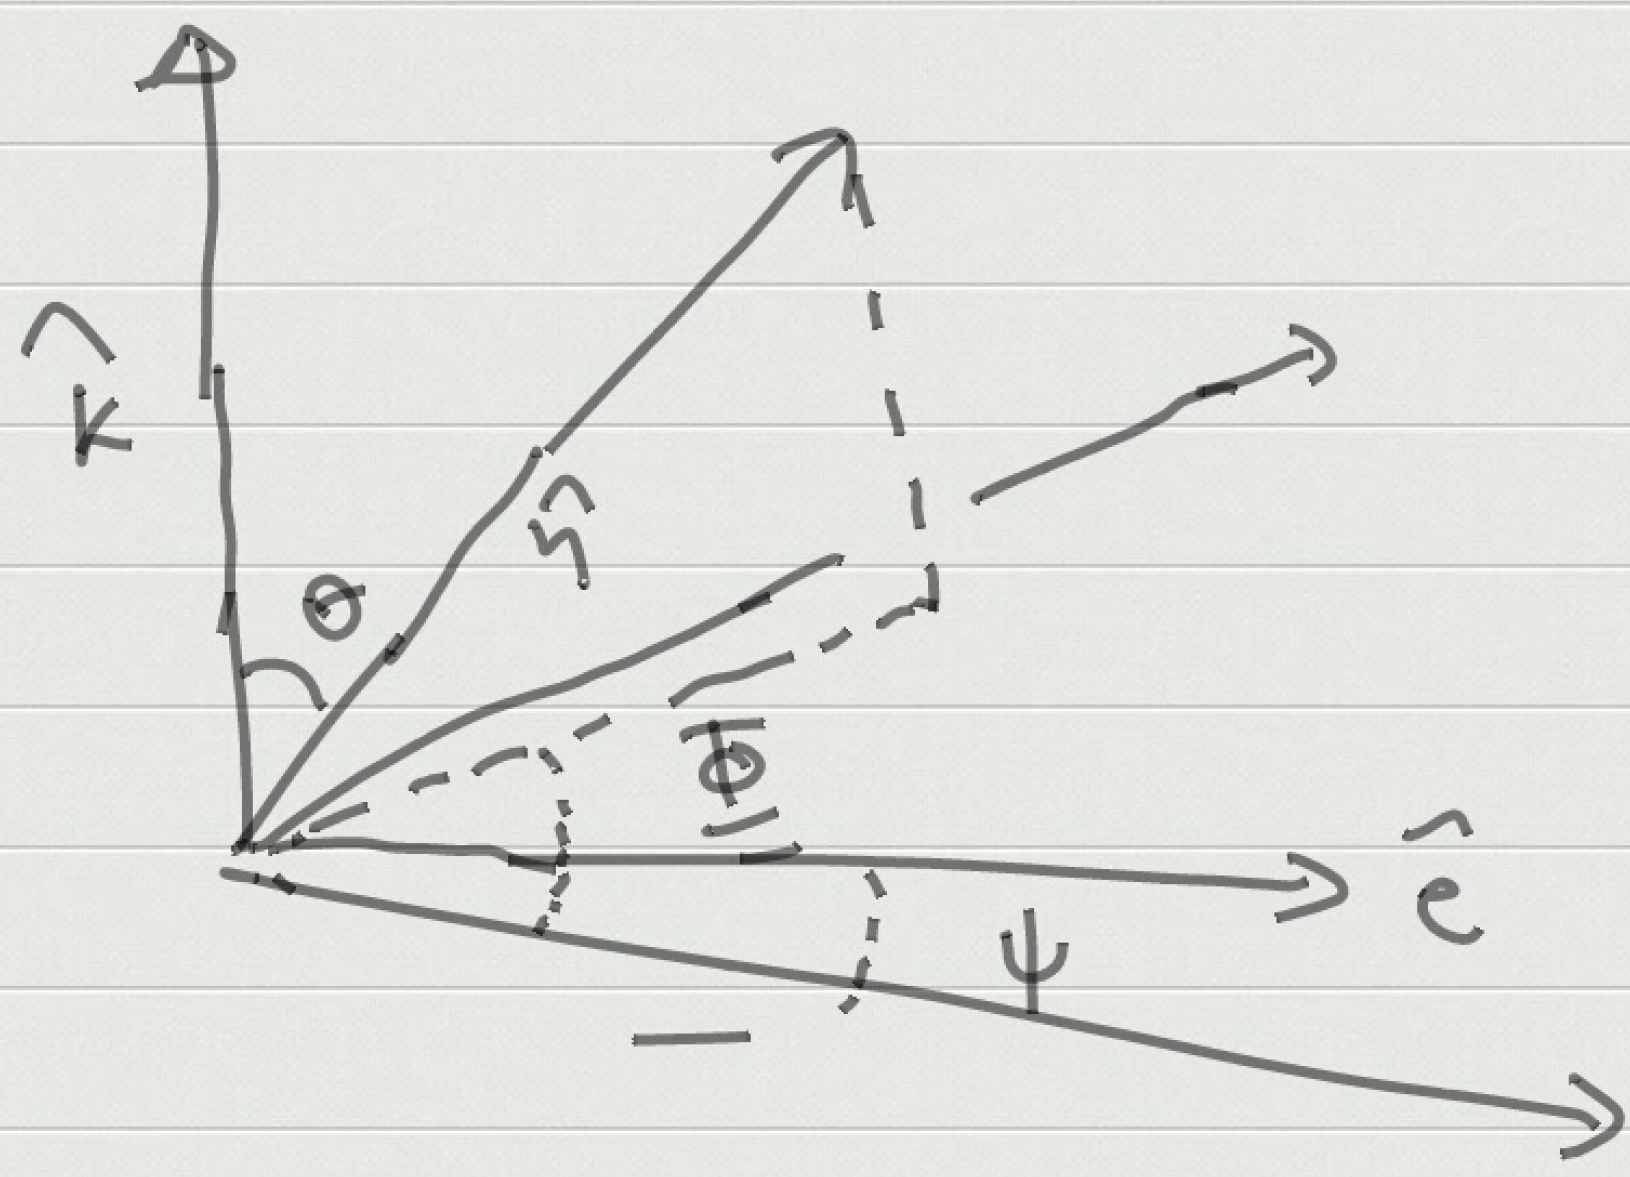
\includegraphics[width=0.9\textwidth]{Pictures/Scattering.png}
\end{minipage}

% \begin{figure}[h]
%     \centering
%     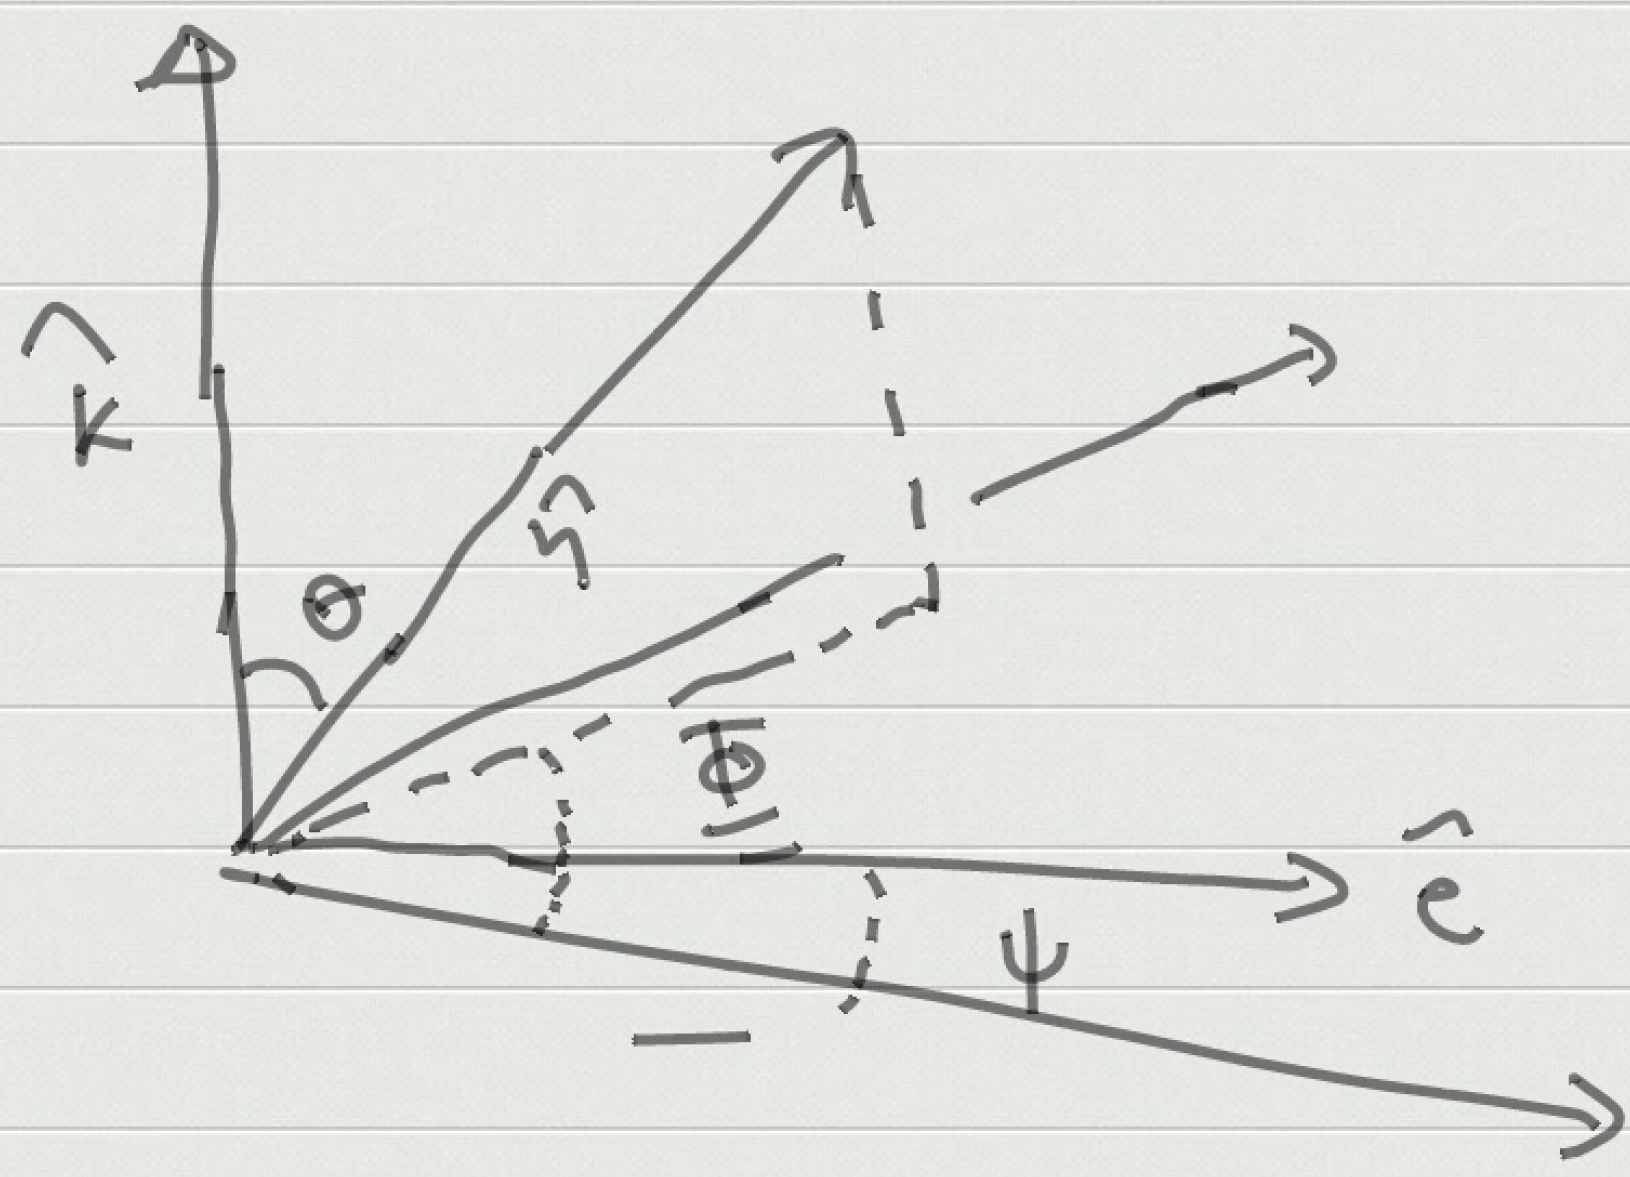
\includegraphics[width=0.2\textwidth]{Pictures/Scattering.png}
% \end{figure}

% The differential cross-section for unpolarised incoming photon beam:
% \begin{align*}
%     \frac{d \sigma}{d \Omega}
%     = \frac{q^4}{16 \pi^2 m^2} \frac{1 + \cos^2(\theta)}{2}
% \end{align*}
% The total cross-section is:
\begin{align*}
    \sigma = \int d \Omega \frac{d \sigma}{d \Omega}
    = \underbrace{\frac{q^4}{16 \pi^2 m^2}}_{\equiv r_q^2} \frac{8 \pi}{3}
    = \frac{8 \pi}{3} r_q^2
\end{align*}

We define the Thomson radius as:
\begin{align*}
    r_e \equiv \frac{e^2}{4 \pi \epsilonnull m_e c^2} \approx 2.8 \cdot 10^{-15} \mathrm{m}
\end{align*}
It can be understood as the effective radius of an electron if you assign to it
a spherical shape.

\subsection{Rayleigh scattering}

Now we examine the scattering of an electromagnetic wave on an electric charge
which is bound in an atom or molecule. The Equations of Motion and its
solution are:
\begin{align*}
    \frac{q E}{m} = \ddot{x} + \gamma \dot{x} + \omega_0^2 x
    \hspace{10pt} \Rightarrow \hspace{10pt}
    \vec{x} = \frac{\frac{q \vec{E}}{m}}{\omega_0^2 - \omega^2 + i \gamma \omega}
\end{align*}
The acceleration is then given as:
\begin{align*}
    \dot{\vec{v}} = \ddot{\vec{x}} = \frac{q \vec{E}}{m} \frac{-\omega^2}{\omega_0^2 - \omega^2 + i \gamma \omega}
    = \dot{\vec{v}}_{Thomson} \frac{-\omega^2}{\omega_0^2 - \omega^2 + i \gamma \omega}
\end{align*}
where $\dot{\vec{v}}_{Thomson} = \frac{q \vec{E}}{m}$. The crosssection is:
\begin{align*}
    \sigma = \sigma_{Thomson} \frac{\omega^4}{(\omega^2 - \omega_0^2)^2 + \gamma^2 \omega^2}
    \hspace{10pt} \text{with} \hspace{10pt}
    \sigma_{Thomson} \equiv \frac{8 \pi}{3} r_q^2
\end{align*}
For $\omega \ll \omega_0$ this process is known as Rayleigh scattering and the
crosssection becomes:
\begin{align*}
    \sigma_{Rayleigh} = \sigma_{Thomson} \frac{\omega^4}{\omega_0^4}
\end{align*}


\section{Electromagnetics in a medium}

We identify two types of motion of charged particles: fast currents within small
distances, due to the motion of charges in atoms and molecules, and slow currents,
which extend at distances much larger than the size of atoms due to free electrons
or ions. In macroscopic measurements we are only interested in slow variations at
the atomic level. We average over the currents within the atoms. We can write:
\begin{align*}
    j^\mu  \approx j_{slow}^\mu + \langle j_{atomic}^\mu \rangle
\end{align*}
We introduce an averaging of a function over some distances via
\begin{align*}
    \langle F(\vec{x},t) \rangle = \int d^3 \vec{y} f(\vec{y}) F(\vec{x}-\vec{y},t)
\end{align*}
where $f(\vec{y})$ is the weighting factor / probability density function. It
is well behaved, smooth, positive, peaks at $0$ and has Norm $1$.

\subsection{Average of the atomic charge density}

The charge density $j_{atomic}^0 = \rho_{atomic}$ corresponds to the charge
density of the charges inside molecules/atoms. We write
\begin{align*}
    \rho_{atomic} = \sum_{n \in \text{ atoms}} \rho_{(n)}
    \hspace{10pt} , \hspace{10pt}
    \rho_{(n)} = \sum_{j \in (n)} q_j \delta(\vec{x} - \vec{x}_n - \vec{x}_j)
\end{align*}
where $\rho_{(n)}$ is the charge density of the $n$-th atom/molecule,
$\vec{x}_n$ is the position of the atom/molecule and $\vec{x}_j$ is the
position of the charge with respect to the "centre" of the molecule.
\begin{align*}
    \langle \rho_{(n)} \rangle &= \sum_{j \in (n)} q_j f(\vec{x} - \vec{x}_n - \vec{x}_j)
    \\
    &= \sum_{j \in (n)} \eckigeklammer{q_j f(\vec{x} - \vec{x}_n) - (q_j \vec{x}_j) \cdot \vec{\nabla}f(\vec{x}-\vec{x}_n) + \dots}
    \\
    &= q_n f(\vec{x} - \vec{x}_n) - \vec{p}_n \cdot \vec{\nabla} f(\vec{x}-\vec{x}_n) + \dots
    \\
    &= q_n f(\vec{x}-\vec{x}_n) - \vec{\nabla} \klammer{\vec{p}_n \cdot f(\vec{x} - \vec{x}_n)} + \dots
\end{align*}
Where we taylor expanded in $\frac{\abs{\vec{x}_j}}{\abs{\vec{x}-\vec{x}_n}}$ and
used that $\vec{\nabla}$ only differentiates with respect to $\vec{x}$. Summing
over all atoms/molecules we can write:
\begin{align*}
    \langle \rho_{atomic} \rangle &\equiv \sum_n \langle \rho_{(n)} \rangle
    = \langle \rho_{eff/atom} \rangle - \vec{\nabla} \cdot \vec{P} + \dots
    \hspace{10pt} \text{with}
    \\
    \langle \rho_{eff/atom} \rangle
    &= \sum_{n \in \text{ atoms}} q_n f(\vec{x} - \vec{x}_n)
    \hspace{10pt} , \hspace{10pt}
    \vec{P} \equiv \sum_{n \in \text{ atoms}} \vec{p}_n \cdot f(\vec{x}-\vec{x}_n)
\end{align*}

\subsection{Average of atomic current density}

We restrict ourselves to non-relativistic velocities. The current density in an
atom/molecule can be written as
\begin{align*}
    \vec{j}_{(n)} = \sum_{k \in n} q_k (\vec{v}_n + \vec{v}_k) \delta(\vec{x} - \vec{x}_n - \vec{x}_k)
\end{align*}
where $\vec{v}_n$ is the velocity of the atom/molecule and $\vec{v}_k$ is the
relative velocity of the charge to the center of the atom.
\begin{align*}
    \langle \vec{j}_n \rangle = \sum_k q_k \klammer{\vec{v}_n + \vec{v}_k}
    f(\vec{x} - \vec{x}_n - \vec{x}_k)
\end{align*}
For $\abs{\vec{x}_k} \ll \abs{\vec{x}_n}$ and $\abs{\vec{v}_n} \ll \abs{\vec{v}_k}$
we can expand:
\begin{align*}
    f(\vec{x} - \vec{x}_n - \vec{x}_k) \approx
    f(\vec{x} - \vec{x}_n) - \vec{x}_k \cdot \vec{\nabla} f(\vec{x} - \vec{x}_n) + \dots
\end{align*}
This yields:
\begin{align*}
    \langle \vec{j}_n \rangle = &\sum_k q_k \vec{v}_k f(\vec{x} - \vec{x}_n)
    + \sum_k q_k \vec{v}_n f(\vec{x} - \vec{x}_n) - \sum_k q_k \vec{v}_k \vec{x}_k \cdot \vec{\nabla} f(\vec{x} - \vec{x}_n)
    \\
    &+ \mathcal{O} \klammer{x_k^2 , x_k v_n , v_n^2}
\end{align*}
We can rewrite:
\begin{align*}
    \sum_k q_k \vec{v}_k f(\vec{x} - \vec{x}_n)
    &\approx \frac{d}{dt} \klammer{\vec{p}_n f(\vec{x} - \vec{x}_n)}
    \\
    \sum_k q_k \vec{v}_k \vec{x}_k \cdot \vec{\nabla} f(\vec{x} - \vec{x}_n)
    &\approx - \vec{\nabla} \times \klammer{\vec{m}_n f(\vec{x} - \vec{x}_n)}
\end{align*}
With $\vec{m}_n$ the magnetic moment of the atom and $\vec{M}$ the magnetization
of the material
\begin{align*}
    \vec{m}_n = \sum_j \frac{q_j}{2} \klammer{\vec{x}_j \times \vec{v}_j}
    \hspace{10pt} , \hspace{10pt}
    \vec{M} = \sum_n \klammer{\vec{m}_n f(\vec{x} - \vec{x}_n)}
\end{align*}
we can write the sum of the average contribution from all atoms as
\begin{align*}
    \langle \vec{j}_{atomic} \rangle &= \sum \langle \vec{j}_{(n)} \rangle
    = \vec{j}_{eff/atomic} + \frac{d \vec{P}}{dt} + \vec{\nabla} \times \vec{M}
    \\
    \vec{j}_{eff/aotmic} &= \sum_n q_n \vec{v}_n f(\vec{x} - \vec{x}_n)
\end{align*}

\subsection{Maxwell equations in a medium}

We approximate the charge and current density as
\begin{align*}
    j^\mu &= j_{free}^\mu + j_{atomic}^\mu \approx j_{free}^\mu + \langle j_{atomic}^\mu \rangle
    \\
    j^0 &\approx \rho_{eff} - \vec{\nabla} \cdot \vec{P} + \dotsb
    \\
    \vec{j} &\approx \vec{j}_{eff} + \frac{\partial \vec{P}}{\partial t} + \vec{\nabla} \times \vec{M} + \dotsb
\end{align*}
With $\vec{M}$ the magnetisation vector. If we substitute into the Maxwell
equations we obtain
\begin{align*}
    \vec{\nabla} \cdot \vec{B} = 0
    \hspace{10pt} &, \hspace{10pt}
    \vec{\nabla} \times \klammer{\vec{B} - \frac{\vec{M}}{c^2 \epsilonnull}}
    = \frac{\vec{j}_{eff}}{c^2 \epsilonnull} + \frac{1}{c^2} \frac{\partial}{\partial t} \klammer{\vec{E} + \frac{\vec{P}}{\epsilonnull}}
    \\
    \vec{\nabla} \times \vec{E} = - \frac{\partial \vec{B}}{\partial t}
    \hspace{10pt} &, \hspace{10pt}
    \vec{\nabla} \cdot \klammer{\vec{E} + \frac{\vec{P}}{\epsilonnull}} = \frac{\rho_{eff}}{\epsilonnull}
\end{align*}
with $\rho_{eff} = \rho_{free} + \rho_{eff/atomic}$ and
$\vec{j}_{eff} = \vec{j}_{free} + \vec{j}_{eff/atomic}$.

\paragraph{The $\vec{D}$ and $\vec{H}$ field}
We define:
\begin{align*}
    \vec{D} \equiv \epsilonnull \vec{E} + \vec{P}
    \hspace{10pt} , \hspace{10pt}
    \vec{H} \equiv \vec{B} - \frac{\vec{M}}{c^2 \epsilonnull}
\end{align*}
Now the Maxwell equations reduce to:
\begin{align*}
    \vec{\nabla} \cdot \vec{D} = \rho
    \hspace{10pt} &, \hspace{10pt}
    \vec{\nabla} \times \vec{E} = - \frac{\partial \vec{B}}{\partial t}
    \hspace{10pt} , \hspace{10pt}
    \vec{\nabla} \cdot \vec{B} = 0
    \\
    \vec{\nabla} \times \vec{H} &= \frac{\vec{j}_{eff}}{\epsilonnull c^2} + \frac{1}{\epsilonnull c^2} \frac{\partial \vec{D}}{\partial t}
\end{align*}

\subsection{Maxwell equations inside a dielectric material}

Assume $\vec{M} = 0$ and $\vec{P} \neq 0$. We find that $\vec{P}$ and $\vec{E}$
are correlated. If we ignore non-linearities we obtain:
\begin{align*}
    \vec{P} = \chi \epsilonnull \vec{E}
\end{align*}
where $\chi$ is the "electric susceptibility". We define:
\begin{align*}
    c_m = \frac{c}{\sqrt{1 + \chi}}
    \hspace{10pt} , \hspace{10pt}
    \epsilon = (1+\chi) \epsilonnull
\end{align*}
Now we can write the Maxwell equations in a dielectric medium as:
\begin{align*}
    \vec{\nabla} \cdot \vec{E}
    \hspace{7pt} , \hspace{7pt}
    \vec{\nabla} \times \vec{E} = - \frac{\partial \vec{B}}{\partial t}
    \hspace{7pt} , \hspace{7pt}
    \vec{\nabla} \cdot \vec{B} = 0
    \hspace{7pt} , \hspace{7pt}
    \vec{\nabla} \times \vec{B} = \frac{\vec{j}_{eff}}{\epsilon c_m^2} + \frac{1}{c_m^2} \frac{\partial \vec{E}}{\partial t}
\end{align*}

\subsection{A model for the dielectric susceptibility $\chi$}

For a dipole we have the differential equation
\begin{align*}
    q \vec{E} = m \klammer{\ddot{x} + \gamma \dot{x} + \omega_0^2 x}
\end{align*}
A solution on the microscopic level is
\begin{align*}
    \vec{x} = \frac{q \vec{E} / m}{\omega_0^2 - \omega^2 + i \omega \gamma}
\end{align*}
So for the dipole moment we obtain:
\begin{align*}
    \vec{P} &= q \vec{x} = \frac{q^2 / m}{\omega_0^2 - \omega^2 + i \omega \gamma} \vec{E}
    \\
    \langle \vec{P} \rangle &= N \vec{x} = \frac{N q^2 / m}{\omega_0^2 - \omega^2 + i \omega \gamma} \vec{E}
\end{align*}
Where $N$ is the density of charges.
When comparing to $\vec{P} = \chi \epsilonnull \vec{E}$ we obtain:
\begin{align*}
    \chi = \chi(\omega) = \frac{\frac{N q^2}{m \epsilonnull}}{\omega_0^2 - \omega^2 + i \omega \gamma}
    = n^2 - 1
\end{align*}
We see that $\chi$ is complex, which has physical consequences on $\epsilon$ and
$c_m$.

\subsection{Waves in a dielectric medium}

If $\vec{j}_{eff} = \rho_{eff} = 0$ ina medium, then we obtain the wave equation
from the Maxwell equations.
\begin{align*}
    \eckigeklammer{\frac{1}{c_m^2} \frac{\partial^2}{\partial t^2} - \vec{\nabla}^2} \vec{E} = 0
\end{align*}
A solution is
\begin{align*}
    \vec{E} = \vec{E}_0 e^{i\klammer{\omega t - \vec{k} \cdot \vec{x}}}
\end{align*}
with $k := \abs{\vec{k}}$:
\begin{align*}
    k^2 = \frac{\omega^2}{c_m^2} = \frac{\omega^2}{c^2} (1+\chi)
    \hspace{10pt} , \hspace{10pt}
    v_{phase} = \frac{\omega}{k} = \frac{c}{n}
    \hspace{10pt} , \hspace{10pt}
    n = \sqrt{1+\chi}
\end{align*}
We see that $n$, the refraction index, is complex.

\subsection{The complex index of refraction}
We can separate the complex and the real part or $n$ into a real and an
imaginary part: $n = n_R - i n_I$. We find that the plane wave propagating
in the dielectric is:
\begin{align*}
    \vec{E} = \vec{E}_0 e^{i \omega \eckigeklammer{t - n \hat{k} \cdot \vec{x}}}
    = \vec{E}_0 e^{i \omega \eckigeklammer{t - \frac{n_R}{c} \hat{k} \cdot \vec{x}}}
    e^{-\omega \frac{n_I}{c} \hat{k} \cdot \vec{x}}
    \hspace{5pt} \Rightarrow \hspace{5pt}
    \abs{\vec{E}} = \abs{\vec{E}_0} e^{- \omega \frac{n_I}{c} \hat{k} \cdot \vec{x}}
\end{align*}

\subsection{Waves in metals}

In metals, electrons move freely at large distances. So we set $\omega_0 = 0$.
\begin{align*}
    \chi(\omega) = \frac{N q^2 / \epsilonnull m}{- \omega^2 + i \omega \gamma}
\end{align*}
The density $N$ can be obtained from macroscopic properties of the metal and
the constant $\gamma$ is an intrinsic parameter of our model. It is related
to the resistanve or its inverse, conductivity. If $\vec{E}$ is constant,
we have a differential equation for $\vec{v}$.
\begin{align*}
    q \vec{E} = m (\dot{\vec{v}} + \gamma \vec{v})
    \hspace{10pt} \Rightarrow \hspace{10pt}
    \vec{v} = \vec{v}_{drift} + \vec{v_0} e^{-\gamma t}
    \hspace{10pt} , \hspace{10pt}
    \vec{v}_{drift} = \frac{q \vec{E}}{m \gamma}
\end{align*}
We further have the relation
\begin{align*}
    \vec{J} = \sigma \vec{E} = N q \vec{v}_{drift} = \frac{N q^2}{m \gamma} \vec{E}
    \hspace{10pt} \Rightarrow \hspace{10pt}
    \gamma = \frac{N q^2}{m \sigma} 
\end{align*}

\subsubsection{Low frequency approximation}

$\omega \rightarrow 0$, so $\omega \gamma \gg \omega^2$. Thus
$n^2 = -i \frac{\sigma}{\epsilonnull \omega} \ \Rightarrow \
\sqrt{\frac{\sigma}{2 \epsilonnull \omega}} (1-i)$ and
$\abs{\vec{E}} = \abs{\vec{E}_0} e^{-\frac{x}{\delta}} \ $ where
$\ \delta = \sqrt{\frac{2 \epsilonnull}{\sigma \omega}} c$.

\subsubsection{High frequency approximation}

$\omega^2 \gg \omega \gamma \ \Rightarrow \ n^2 \approx 1 - \frac{\omega_P^2}{\omega^2} \ $
where $\ \omega_P^2 = \frac{N q^2}{m \epsilonnull}$ is the so called "plasma
frequency". If $\omega < \omega_P$, then $n \in i \R$ and therefore the waves
die off after some length. If $\omega > \omega_P$, then $n \in \R$ and thus the
metal becomes transparent to the electromagnetic wave.

\subsection{Reflection and refraction}

Consider two materials with refraction indices $n_1$ and $n_2$ separated by a
boundary surface on the $yz$ plane. For the electromagnetic fields we have:
% We want to analyse Maxwells equations on the
% boundary to gain some insight on the fields.
% \begin{align*}
%     \partial_x E_x + \partial_y F_y + \partial_z E_z
%     = \vec{\nabla} \cdot \vec{E}
%     = - \frac{1}{\epsilonnull} \vec{\nabla} \cdot \vec{P}
%     = - \frac{1}{\epsilonnull} \klammer{\partial_x P_x + \partial_y P_y + \partial_z P_z}
% \end{align*}
% The derivatives in $x$-direction are much bigger than the other ones, thus
% we obtain:
% \begin{align*}
%     \partial_x E_x = - \frac{1}{\epsilonnull} \partial_x P_x
%     \ &\Rightarrow \
%     \frac{E_{x,2} - E_{x,1}}{\Delta x} = - \frac{1}{\epsilonnull} \frac{P_{x,2} - P_{x,1}}{\Delta x}
%     \\ &\Rightarrow \
%     \epsilonnull E_{x,2} + P_{x,2} = \epsilonnull E_{x,1} + P_{x,1}
% \end{align*}
% Further, with again using that the derivatives with respect to $x$ is much
% larger than the other ones we obtain:
% \begin{align*}
%     \vec{\nabla} \times \vec{E} = - \frac{\partial \vec{B}}{\partial t}
%     \ \Rightarrow \
%     \frac{\partial E_x}{\partial z} - \frac{\partial E_z}{\partial x} = - \frac{\partial B_y}{\partial t}
%     \ \rightsquigarrow \
%     \frac{\partial E_z}{\partial x} = 0
%     \ \rightarrow \
%     E_{z,1} = E_{z,2}
% \end{align*}
% Similarly we obtain $E_{y,1} = E_{y,2}$ and from the other Maxwell eq we obtain
% $\vec{B}_2 = \vec{B_1}$ so in conclusion:
\begin{align*}
    \vec{B}_1 = \vec{B}_2
    \hspace{10pt} , \hspace{10pt}
    \vec{E}_{1,\parallel} = \vec{E}_{2,\parallel}
    \hspace{10pt} , \hspace{10pt}
    \klammer{\epsilonnull \vec{E}_1 + \vec{P}_1}_\perp = \klammer{\epsilonnull \vec{E}_2 + \vec{P}_2}_{\perp}
\end{align*}

\subsubsection{Snell's law}

Consider an incident electromagnetic plane-wave $(\vec{E}_I,\vec{B}_I)$ from
a medium $n_1$ to a medium $n_2$, the reflected $(\vec{E}_R,\vec{B}_R)$ and transmitted
electromagnetic field $(\vec{E}_T,\vec{B}_T)$. The following are true:
\begin{align*}
    \vec{E}_1 &= \vec{E}_I + \vec{E}_R
    \hspace{10pt} , \hspace{10pt}
    \vec{E}_2 = \vec{E}_T
    \hspace{10pt} , \hspace{10pt}
    \vec{B}_1 = \vec{B}_I + \vec{B}_R
    \hspace{10pt} , \hspace{10pt}
    \vec{B}_2 = \vec{B}_T
    \\
    \vec{E}_I &= \hat{e}_I E_I e^{i(\omega_I t - \vec{k}_I \cdot \vec{x})}
    \hspace{5pt} , \hspace{5pt}
    \vec{E}_R = \hat{e}_R E_R e^{i(\omega_R t - \vec{k}_R \cdot \vec{x})}
    \\
    \vec{E}_T &= \hat{e}_T E_T e^{i(\omega_T t - \vec{k}_T \cdot \vec{x})}
    \\
    \vec{B}_I &= \frac{\vec{k}_I \times \vec{E}_I}{\omega_I}
    \hspace{10pt} , \hspace{10pt}
    \vec{B}_R = \frac{\vec{k}_R \times \vec{E}_R}{\omega_R}
    \hspace{10pt} , \hspace{10pt}
    \vec{B}_T = \frac{\vec{k}_T \times \vec{E}_T}{\omega_T}
    \\
    \vec{k}_I \cdot \hat{e}_I &= \vec{k}_R \cdot \hat{e}_R
    = \vec{k}_T \cdot \hat{e}_T = 0
    \\
    \frac{k_I}{\omega_I} &= \frac{k_R}{\omega_R} = \frac{n_1}{c}
    \hspace{10pt} , \hspace{10pt}
    \frac{k_T}{\omega_T} = \frac{n_2}{c}
\end{align*}
With some boundary conditions we obtain:
\begin{align*}
    \omega_I = \omega_R = \omega_T = \omega
    \hspace{10pt} \text{and} \hspace{10pt}
    \vec{k}_{I,\parallel} = \vec{k}_{R,\parallel} = \vec{k}_{T,\parallel}
    = \vec{k}_{\parallel}
\end{align*}
We also obtain Snell's law
\begin{align*}
    \theta_I = \theta_R
    \hspace{10pt} , \hspace{10pt}
    \sin(\theta_T) = \frac{n_1}{n_2} \sin(\theta_I)
\end{align*}




\end{document}